\documentclass[slidescentered]{beamer}

\usepackage{tikz}
\usetikzlibrary{backgrounds,fit, positioning,shapes}
\usepackage{mathtools}
\newlength{\NOTskip} 
\def\NOT#1{\settowidth{\NOTskip}{\ensuremath{#1}}%
	\hspace{0.5\NOTskip}\mathclap{\not}\hspace{-0.5\NOTskip}#1}
\usepackage{url}
\def\UrlBreaks{\do\/\do-}
\usepackage{caption}
\newcommand{\source}[1]{\caption*{\tiny Adapted from: {#1}} }
\usepackage[absolute,overlay]{textpos}


\mode<presentation>
{
	\usetheme{default}      % or try Darmstadt, Madrid, Warsaw, ...
	\usecolortheme{default} % or try albatross, beaver, crane, ...
	\usefonttheme{default}  % or try serif, structurebold, ...
	\setbeamertemplate{navigation symbols}{}
	\setbeamertemplate{caption}[numbered]
} 

\addtobeamertemplate{navigation symbols}{}{%
	\usebeamerfont{footline}%
	\usebeamercolor[fg]{footline}%
	\hspace{1em}%
	\insertframenumber/\inserttotalframenumber
}

\newcommand{\backupbegin}{
	\newcounter{framenumberappendix}
	\setcounter{framenumberappendix}{\value{framenumber}}
}
\newcommand{\backupend}{
	\addtocounter{framenumberappendix}{-\value{framenumber}}
	\addtocounter{framenumber}{\value{framenumberappendix}} 
}

\newsavebox{\authbox}
\sbox{\authbox}{%
	\centering
	\begin{minipage}{0.45\linewidth}
		\centering\normalsize
		\textit{Author}: \par
		Giona Soldati
	\end{minipage}
	\hfill
	\begin{minipage}{0.45\linewidth}
		\centering\normalsize
		\textit{Supervisors}: \par
		Daniele Marazzina \\
		Ferdinando M. Ametrano
	\end{minipage}
}


\title{An Advanced Signature Scheme:}
\subtitle{Schnorr Algorithm and its Benefits to the Bitcoin Ecosystem}
\author[Giona Soldati]{%
	\usebox{\authbox}
}

\bigskip

\institute{School of Industrial and Information Engineering \\
	Master of Science in Mathematical Engineering}
\date{20$^{\text{th}}$ December 2018}
\titlegraphic{%
	\begin{picture}(0,0)
	\put(30, 230){\makebox(0,0)[rt]{\includegraphics[width=2cm]{images/polimi.png}}}
	\end{picture}}

\setbeamertemplate{bibliography entry title}{}
\setbeamertemplate{bibliography entry location}{}

\begin{document}
	\AtBeginSection[]{
	\begin{frame}{Outline}
		\small \tableofcontents[currentsection, hideothersubsections]
	\end{frame} 
	}

    \begin{frame}
        \maketitle
    \end{frame}
	
	\begin{frame}{Introduction}
	The Elliptic Curve Digital Signature Algorithm (ECDSA) is used in the Bitcoin protocol as signature scheme, but it has some problems:
		\begin{enumerate}
			\item Limited efficiency (DER encoding, no batch validation, modular inversion);
			\item Poor implementation of higher level constructions (low privacy and fungibility, limited scalability);
			\item Not provably secure (malleable).
		\end{enumerate}
	\end{frame}

    \section{Mathematical background and cryptographic primitives}
    
    \subsection{Hash functions}
    \begin{frame}{Hash functions ($\simeq$ Random Oracle)}
    		\begin{center}
    			\begin{tikzpicture}[
    			every node/.style = {% is not necessary, default node's shape is rectangle
    				align=center}
    			]
    			\tikzstyle{bigbox} = [draw=blue!50, thick, fill=blue!10, rounded corners, rectangle]
    			\tikzstyle{box} = [minimum size=0.6cm, rounded corners,rectangle, fill=blue!50]
    			
    			\node (title1) [draw] {Input};
    			
    			\node (a) [below=of title1, yshift=0.5cm] {``Politecnico \\ di Milano"};
    			\node (b) [below=of a, yshift=0.5cm] {\includegraphics[scale=0.2]{images/divina.jpg}};
    			\node (c) [below=of b, yshift=0.5cm] {\includegraphics[scale=0.07]{images/film.jpg}};
    			
    			\begin{pgfonlayer}{background}
    			\node[bigbox] [fit = (a) (c)] {};
    			\end{pgfonlayer}
    			
    			\node[xshift=3.4cm] (title2) [draw, right=of title1] {Output};
    			
    			\node (d) [draw, right=of a, xshift = 0.5cm] {52c61456bd3d60c08599a8c61e113e7b \\ c39118b75d06b2643c55957ece91269b};
    			\node (e) [draw, right=of b, xshift=0.7cm] {1f12f8384d5941e8e273926635be646a \\ f786405a8662e0ba6dd1fd0526ec0528};
    			\node (f) [draw, right=of c, xshift=0.3cm] {721a14d89cb463b51cf20ecc707aa290 \\ 5b7c8f32d9114dc19fe353e611494bf1};
    			
    			\begin{pgfonlayer}{background}
    			\node[bigbox] [fit = (d) (f)] {};
    			\end{pgfonlayer}
    			

    			\node[xshift=1.9cm, yshift=-1.2cm] (z) {$\xrightarrow{\ \ \ \ \ \ \ \ \ \ \ }{}$};
    			\node[xshift=1.8cm, yshift=-1.5cm] (z) {$\NOT{\xleftarrow{\ \ \ \ \ \ \ \ \ \ \ }}{}$};
    			\node[xshift=1.8cm, yshift=-3.4cm] (z) {$\xrightarrow{\ \ \ \ \ \ \ \ \ \ \ \ }{}$};
    			\node[xshift=1.7cm, yshift=-3.7cm] (z) {$\NOT{\xleftarrow{\ \ \ \ \ \ \ \ \ \ \ \ }}{}$};
    			\node[xshift=2cm, yshift=-6.2cm] (z) {$\xrightarrow{\ \ \ \ \ \ \ \ \ }{}$};
    			\node[xshift=1.9cm, yshift=-6.5cm] (z) {$\NOT{\xleftarrow{\ \ \ \ \ \ \ \ \ }}{}$};

    			
    			\node (g) [right=of d, xshift = -0.9cm] {\includegraphics[scale=0.14]{images/fingerprint1.jpg}};
    			\node (g) [right=of e, xshift = -0.7cm] {\includegraphics[scale=0.24]{images/fingerprint2.jpg}};
    			\node (g) [right=of f, xshift = -0.8cm] {\includegraphics[scale=0.02]{images/fingerprint3.jpg}};
    			
    			\node (h) [right=of a, xshift = -0.7cm, yshift = 0.3cm] {\tiny SHA-256};
    			\node (h) [right=of b, xshift = -0.5cm, yshift = 0.3cm] {\tiny SHA-256};
    			\node (h) [right=of c, xshift = -0.95cm, yshift = 0.3cm] {\tiny SHA-256};
    			\end{tikzpicture}
    		\end{center}
		\end{frame}

		\subsection{Elliptic curve cryptography}
		\begin{frame}{Elliptic curve cryptography}
			\begin{columns}
				\begin{column}{0.5\linewidth}
					An elliptic curve over a finite field is defined by the equation: 
					$$E(\mathbb{F}_p): \ y^2 = x^3 + ax + b \ (\text{mod} \ p).$$
					It is possible to define:
					\begin{itemize}
						\item \hyperlink{point_addition}{Addition}: \\
						$Q_3 := Q_1 + Q_2,$ 
						\\$\forall Q_1, Q_2 \in E(\mathbb{F}_p)$;
						\item Scalar multiplication: \\
						$nG := G + ... + G$, $\forall G \in E(\mathbb{F}_p),$ $\forall n \in \mathbb{N}$.
					\end{itemize}
			\end{column}
			\begin{column}{0.6\linewidth}
				\begin{tikzpicture}[
					every node/.style = {% is not necessary, default node's shape is rectangle
					align=center}
					]
				
					\node () at (0,0) {};
					\node (a) [xshift = 2.3cm] {\includegraphics[height=5cm, width=6.4cm]{images/ec_over_ff}};
				
					\node (b) [below=of a, yshift = 1.2cm] {\small The curve $y^2 = x^3 - x \ \text{over} \ \mathbb{F}_{61}$.};
				\end{tikzpicture}
			\end{column}
		\end{columns}
	\end{frame}

    
    \begin{frame}{Discrete logarithm problem}
    	Fixed $G \in E(\mathbb{F}_p)$, we can define $Q = qG \ \ \forall q \in \{1, ..., n - 1\}$,  where $n$ is the smallest integer such that $nG = \infty$, the identity element of the sum:
    	\begin{itemize}
    		\item The direct operation $q \mapsto Q$ is efficient (\hyperlink{double_add}{double and add algorithm});
    		\item The inverse operation $Q \mapsto q$ is computationally infeasible for certain groups.
    	\end{itemize}
    	
    	\bigskip
    	\noindent
    	Asymmetric cryptography: $\{\textcolor{red}{q}, \textcolor{green}{Q}\}$ is a key pair whose elements have complementary roles.
    	\begin{itemize}
    		\item $\textcolor{red}{q}$: private key (signature);
    		\item $\textcolor{green}{Q}$: public key (verification).
    	\end{itemize}
	\end{frame}
    
    \section{Digital signature schemes}
    
    \begin{frame}{Digital signature}
        \begin{center}
        	\begin{tikzpicture}[
        	every node/.style = {% is not necessary, default node's shape is rectangle
        		align=center}
        	]
        	
        	\node (a) {\includegraphics[scale=0.2]{images/Alice.jpg}};
        	\node (b) [text width=3cm, below=of a, yshift=1cm] {Alice};
        	
        	\node (d) [right=of a] {\includegraphics[scale=0.25]{images/Bob.jpg}};
        	\node (e) [text width=3cm, below=of d, yshift=1cm] {Bob};
        	
        	\node<1-4> (c) [xshift=2.1 cm, yshift=-1cm] {\includegraphics[scale=0.1]{images/sig.jpg}};
        	\node<1> (f) [xshift = 2.1 cm, yshift = 1cm] {\includegraphics[scale=0.055]{images/doc.png}};
        	\node<2-> (f) [xshift = 2.1 cm, yshift = 1cm] {\includegraphics[scale=0.1]{images/bitcoin.png}};
        	\node<5> (c) [xshift=2.1 cm, yshift=-1cm] {\includegraphics[scale=0.1]{images/bitcoin_sig.jpg}};

        	
        	\node<3> (f) [xshift = -1.2 cm, yshift = 1cm] {$q_A$};
        	\node<3> (f) [xshift = 5.5 cm, yshift = 1cm] {$Q_A$};
        	\node<4-> (f) [xshift = -1.2 cm, yshift = 1cm] {\textcolor{red}{$q_A$}};
        	\node<4-> (f) [xshift = 5.5 cm, yshift = 1cm] {\textcolor{green}{$Q_A$}};
        	
        	
        	
        	
        	\draw [->] (a) -- (d);
        	\end{tikzpicture}
        	\begin{itemize}
        		\item<3-> Authentication: the recipient is confident that the message comes from the alleged sender;
        		\item<4-> Non repudiation: the sender cannot deny having sent the message;
        		\item<5> Integrity: ensures that the message has not been altered during transmission.
        	\end{itemize}
        \end{center}
    \end{frame}

	\subsection{ECDSA}
	\begin{frame}{Elliptic curve digital signature algorithm}
		\begin{columns}
			\begin{column}{0.6\linewidth}
				ECDSA\_SIG$(m, q)$:
				\begin{enumerate}
					\item<3 -> $z \gets \text{hash}(m)$;
					\item<4 -> $k \xleftarrow{\text{\$}} \{1, ..., n - 1\}$;
					\item<5 -> $K \gets kG$;
					\item<6 -> $r \gets x_K \ (\text{mod} \ n)$;
					\item<7 -> $s \gets k^{-1}(z + rq) \ (\text{mod} \ n)$;
					\item<8 -> \textbf{return} $(r, s)$.
				\end{enumerate}
			\end{column}
			\begin{column}{0.5\linewidth}
				\begin{figure}
				\only<1> {\vspace*{-0.7cm}
					\hspace*{-1.7cm}
					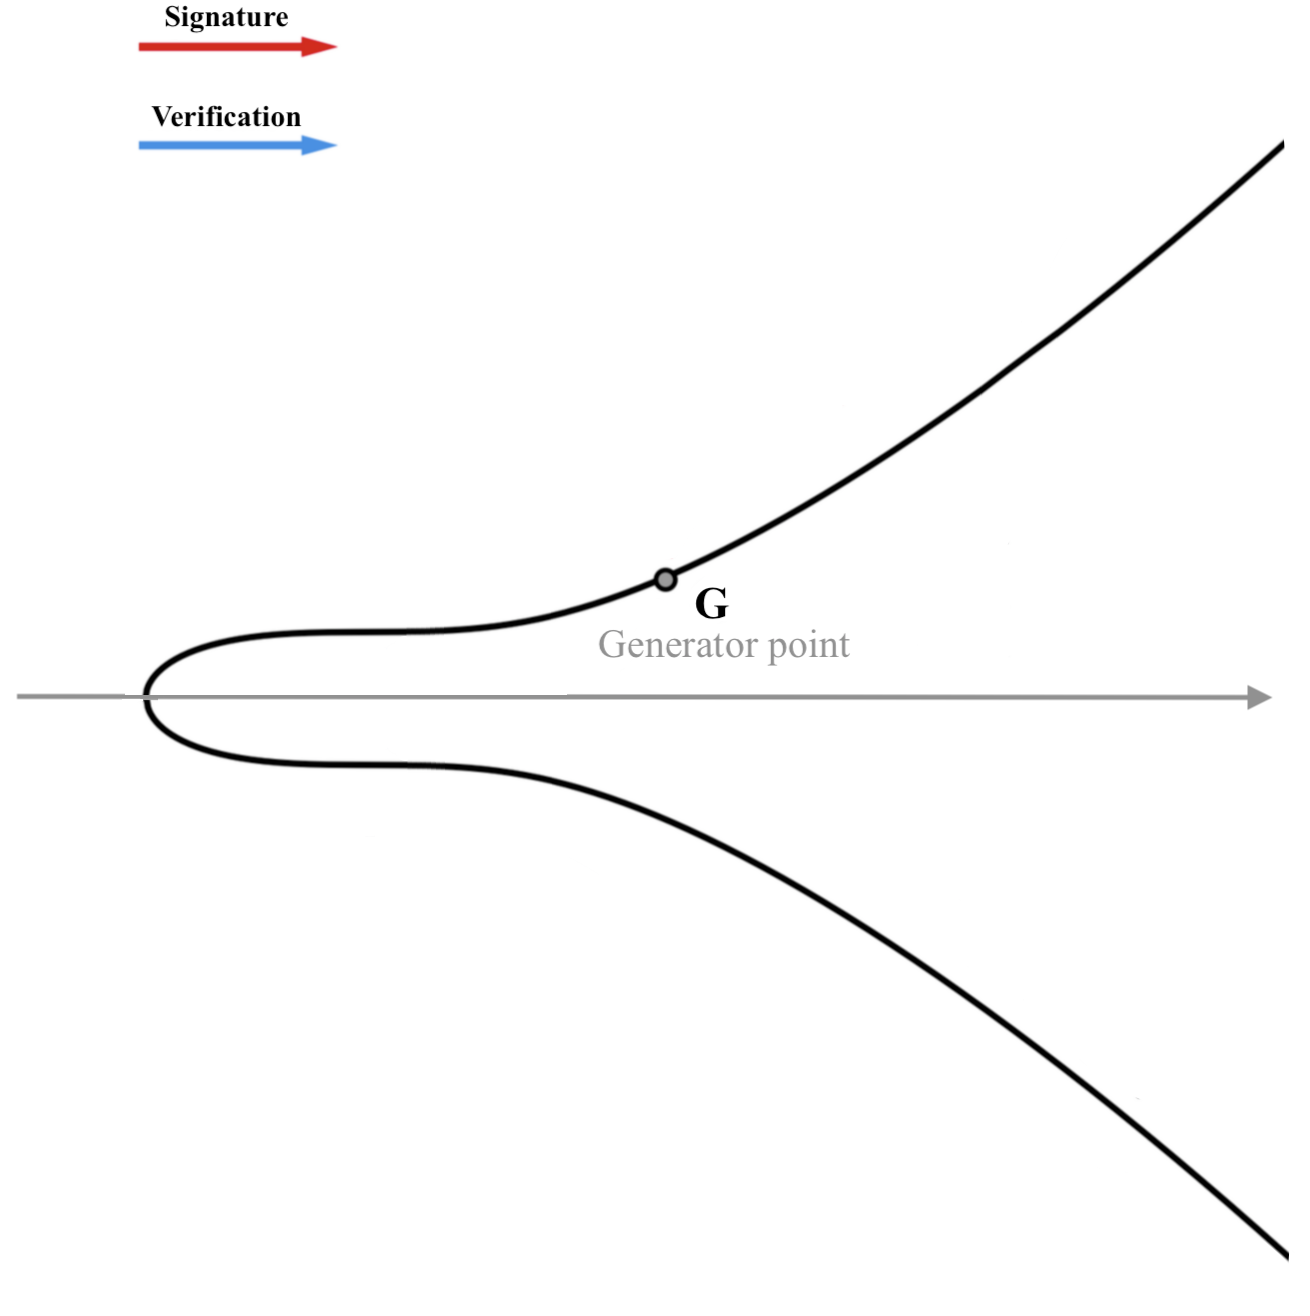
\includegraphics[scale=0.29]{images/ECDSA1}
				\source{\tiny \url{https://medium.com/cryptoadvance/how-schnorr-signatures-may-improve-bitcoin-91655bcb4744}}}
				\only<2-4> {\vspace*{-0.7cm}
					\hspace*{-1.7cm}
					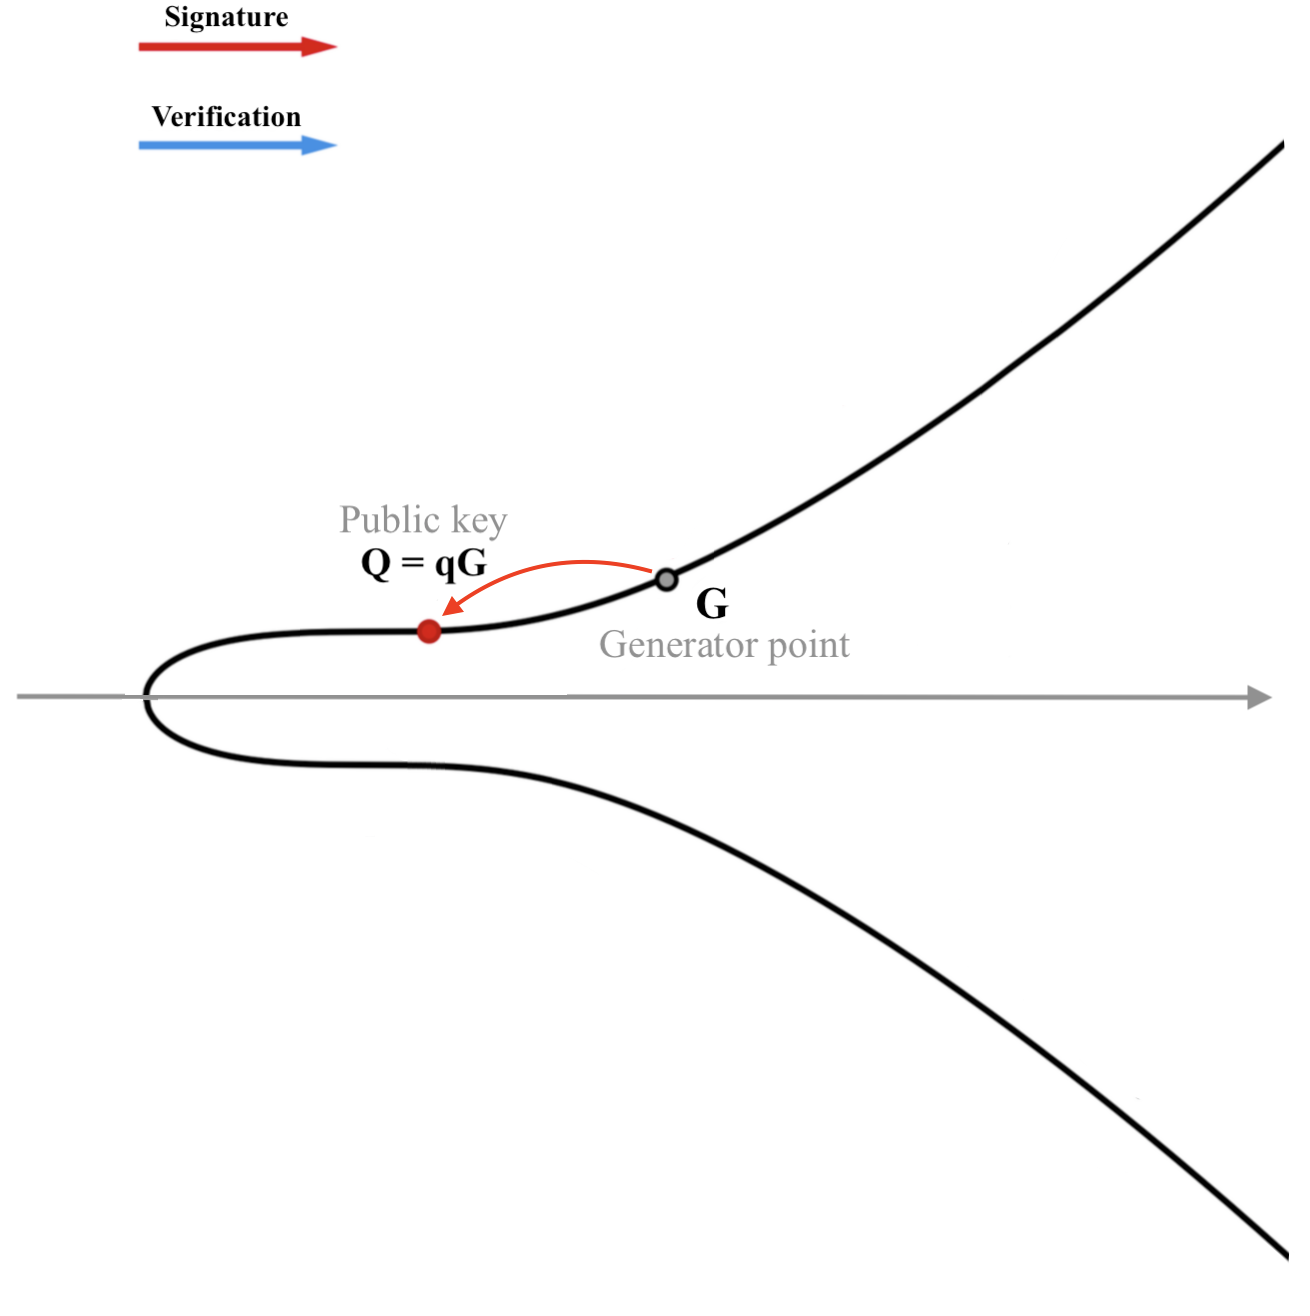
\includegraphics[scale=0.29]{images/ECDSA2}
				\source{\tiny \url{https://medium.com/cryptoadvance/how-schnorr-signatures-may-improve-bitcoin-91655bcb4744}}}
				\only<5> {\vspace*{-0.7cm}
					\hspace*{-1.7cm}
					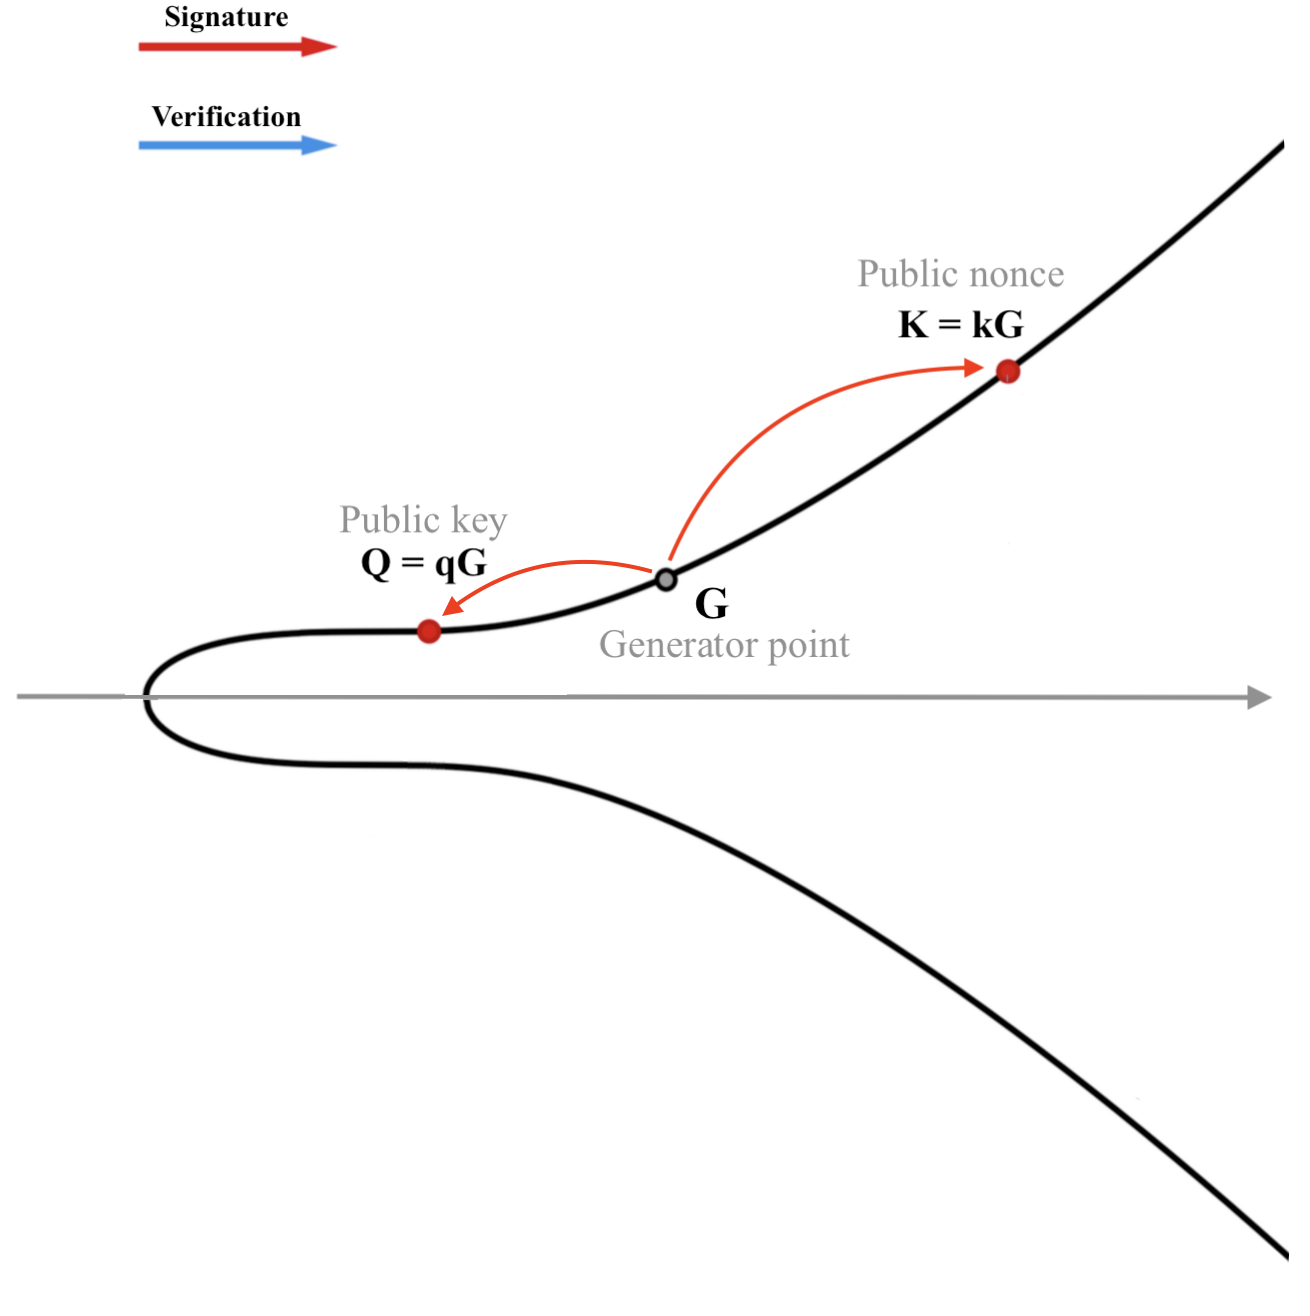
\includegraphics[scale=0.29]{images/ECDSA3}
				\source{\tiny \url{https://medium.com/cryptoadvance/how-schnorr-signatures-may-improve-bitcoin-91655bcb4744}}}
				\only<6-8> {\vspace*{-0.7cm}
					\hspace*{-1.7cm}
					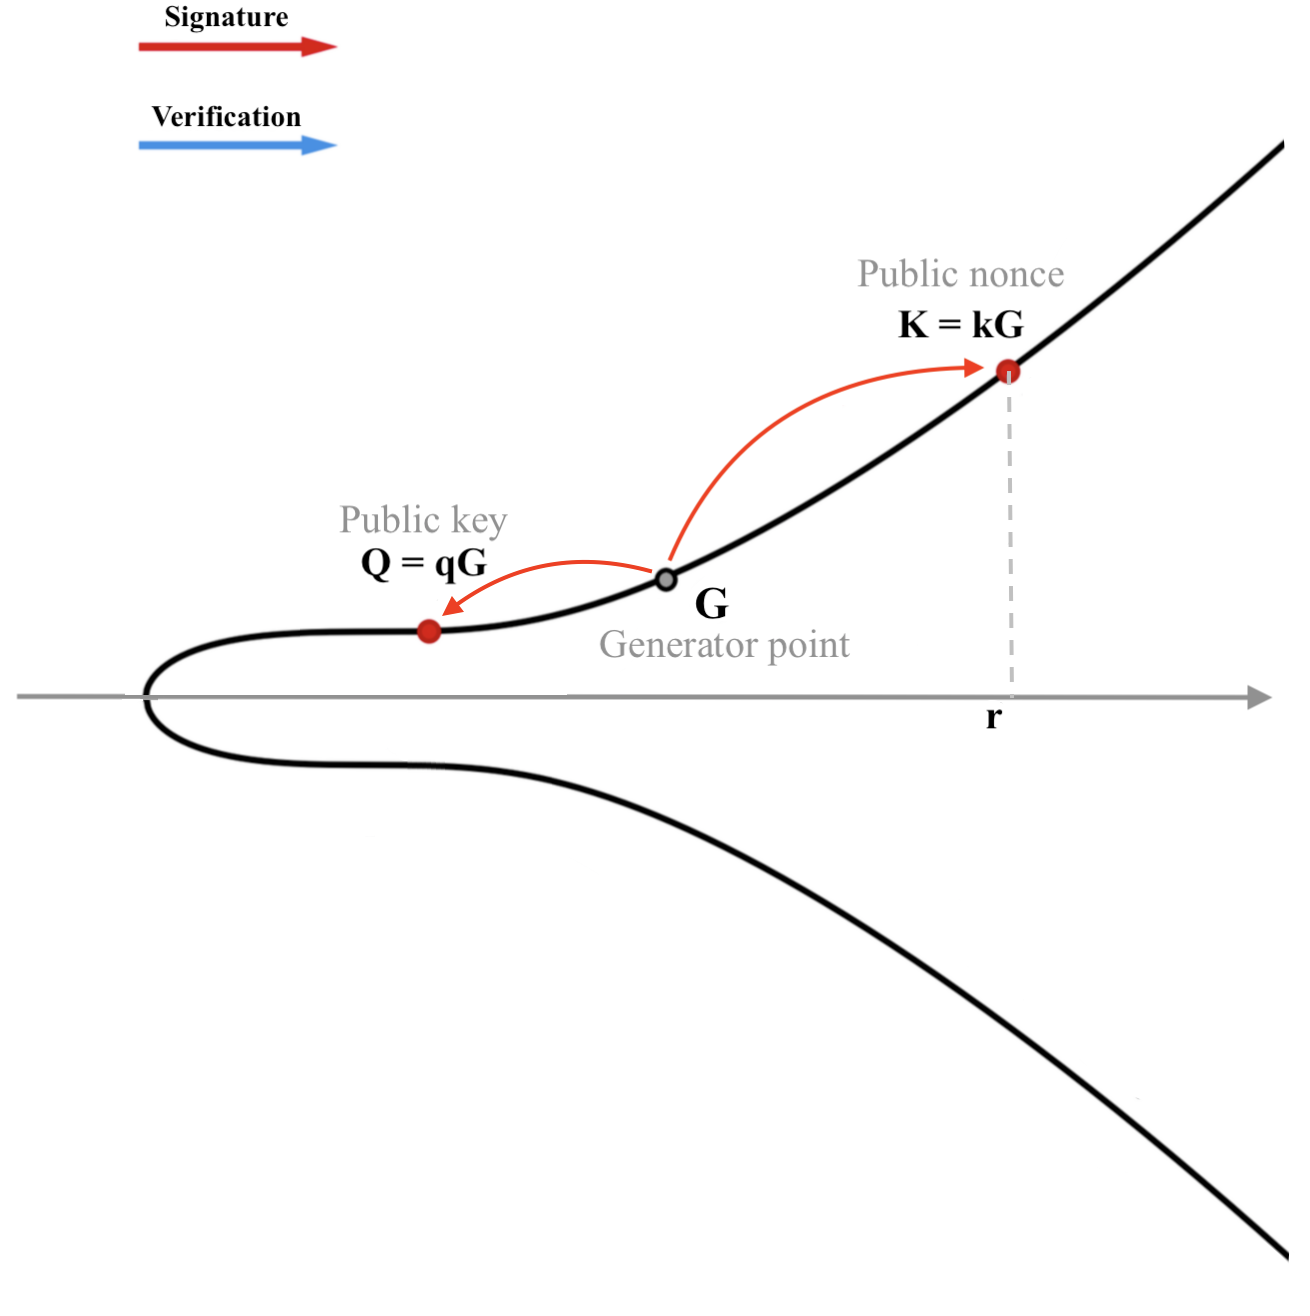
\includegraphics[scale=0.29]{images/ECDSA4}
				\source{\tiny \url{https://medium.com/cryptoadvance/how-schnorr-signatures-may-improve-bitcoin-91655bcb4744}}}
				\end{figure}
			\end{column}
		\end{columns}
	\end{frame}

	\begin{frame}{Elliptic curve digital signature algorithm}
		\begin{columns}
			\begin{column}{0.6\linewidth}
				ECDSA\_VER$((r,s), m, Q)$:
				\begin{enumerate}
					\item<2 -> \textbf{If} $r \notin \{1, ..., n - 1\}$ \textbf{or} $s \notin \{1, ..., n - 1\}$: \\ \textbf{\ \ \ return False};
					\item<3 -> $z \gets \text{hash}(m)$;
					\item<4 -> $u_1 \gets zs^{-1} \ (\text{mod} \ n)$, $u_2 \gets rs^{-1} \ (\text{mod} \ n)$;
					\item<5 -> $K \gets u_1G + u_2Q$;
					\item<8 -> \textbf{return $r = x_K \ (\text{mod} \ n)$}.
				\end{enumerate}
			\end{column}
			\begin{column}{0.5\linewidth}
				\begin{figure}
					\only<1-4> {\vspace*{-0.7cm}
						\hspace*{-1.7cm}
						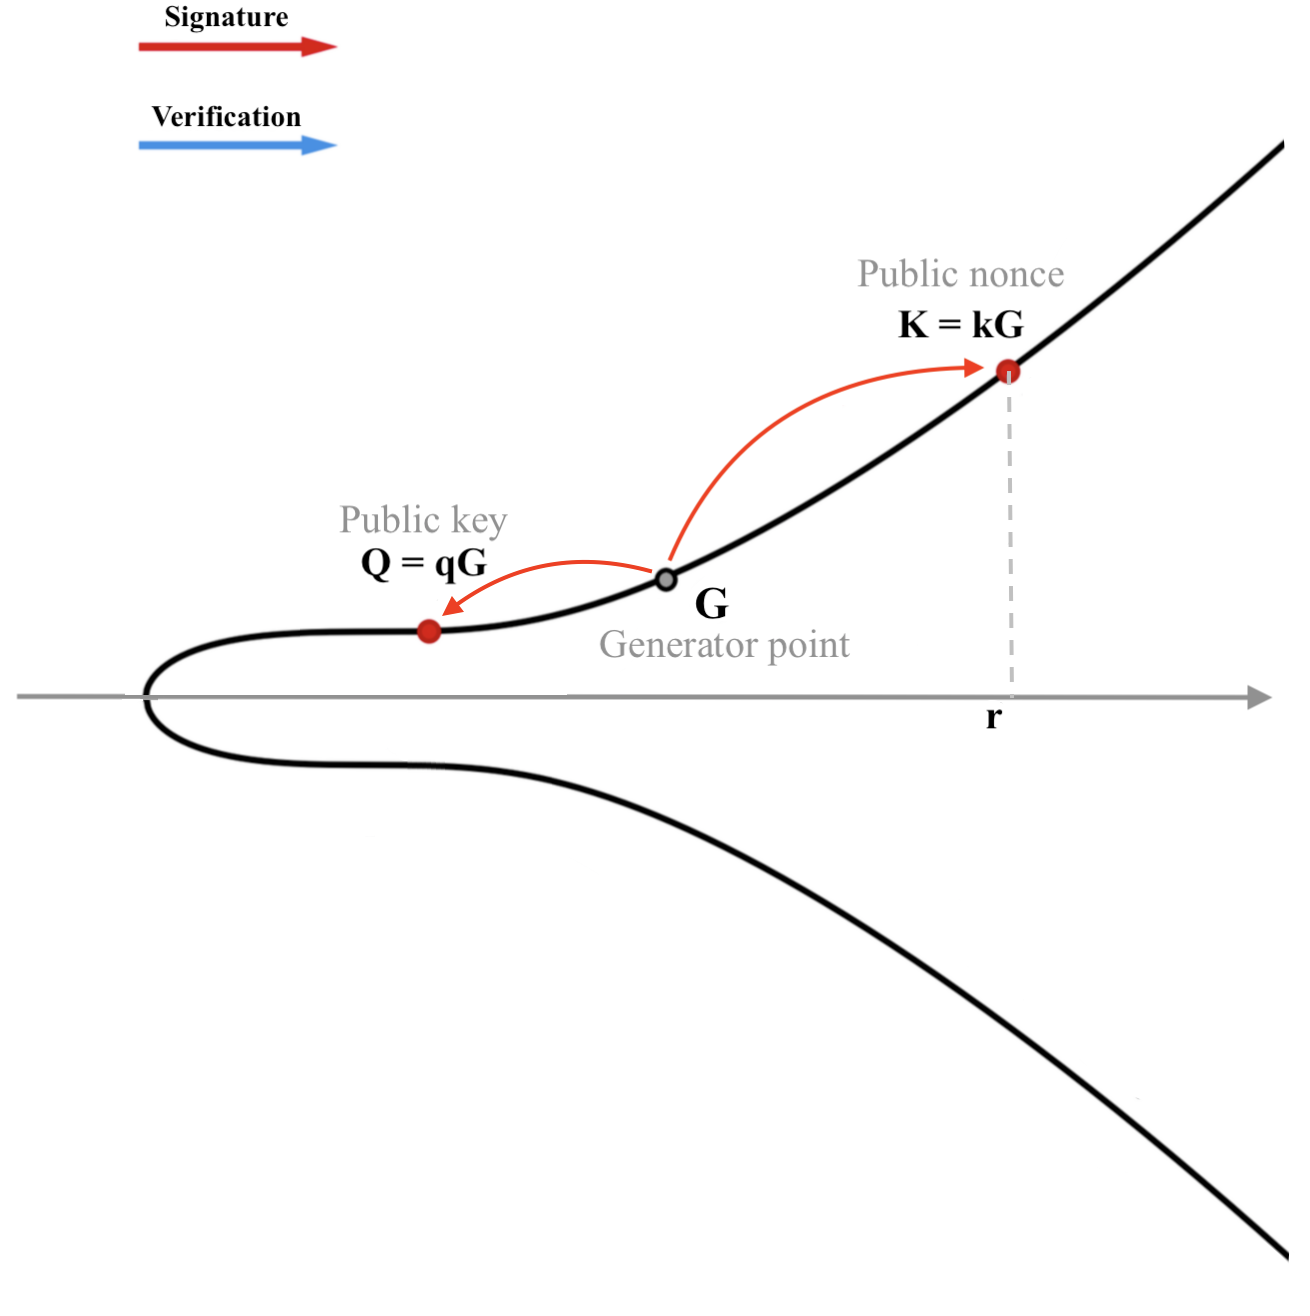
\includegraphics[scale=0.29]{images/ECDSA4}
						\source{\tiny \url{https://medium.com/cryptoadvance/how-schnorr-signatures-may-improve-bitcoin-91655bcb4744}}}
					\only<5> {\vspace*{-0.7cm}
						\hspace*{-1.7cm}
						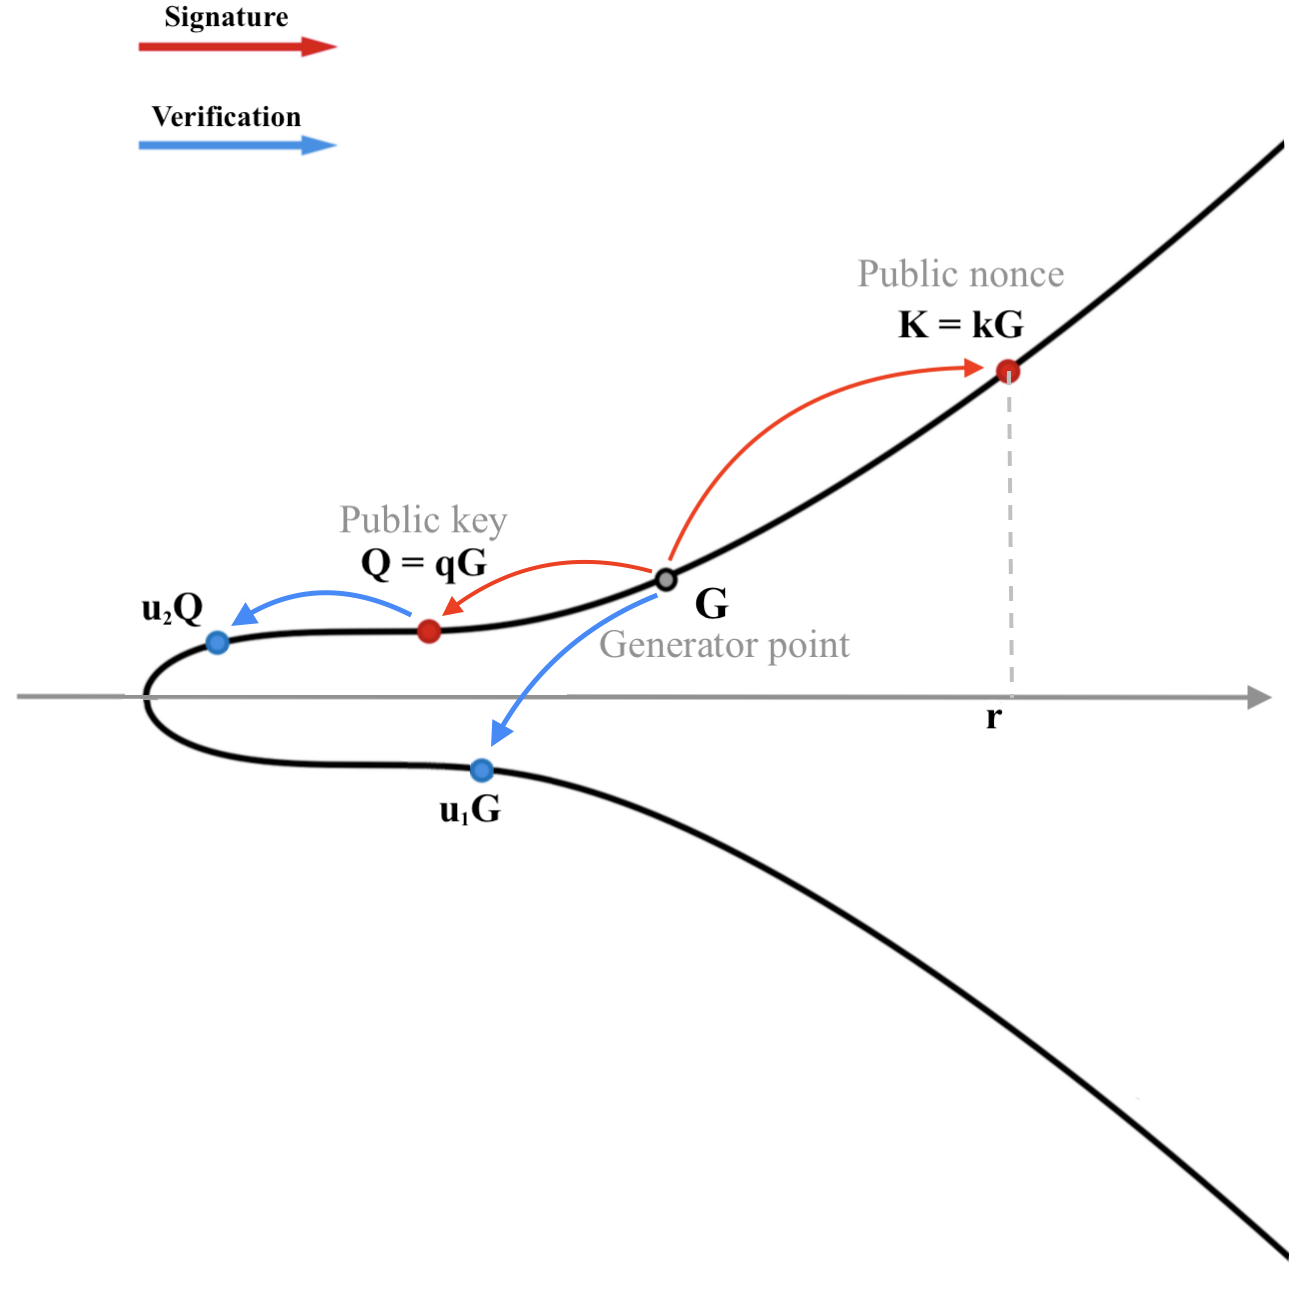
\includegraphics[scale=0.29]{images/ECDSA5}
						\source{\tiny \url{https://medium.com/cryptoadvance/how-schnorr-signatures-may-improve-bitcoin-91655bcb4744}}}
					\only<6> {\vspace*{-0.7cm}
						\hspace*{-1.7cm}
						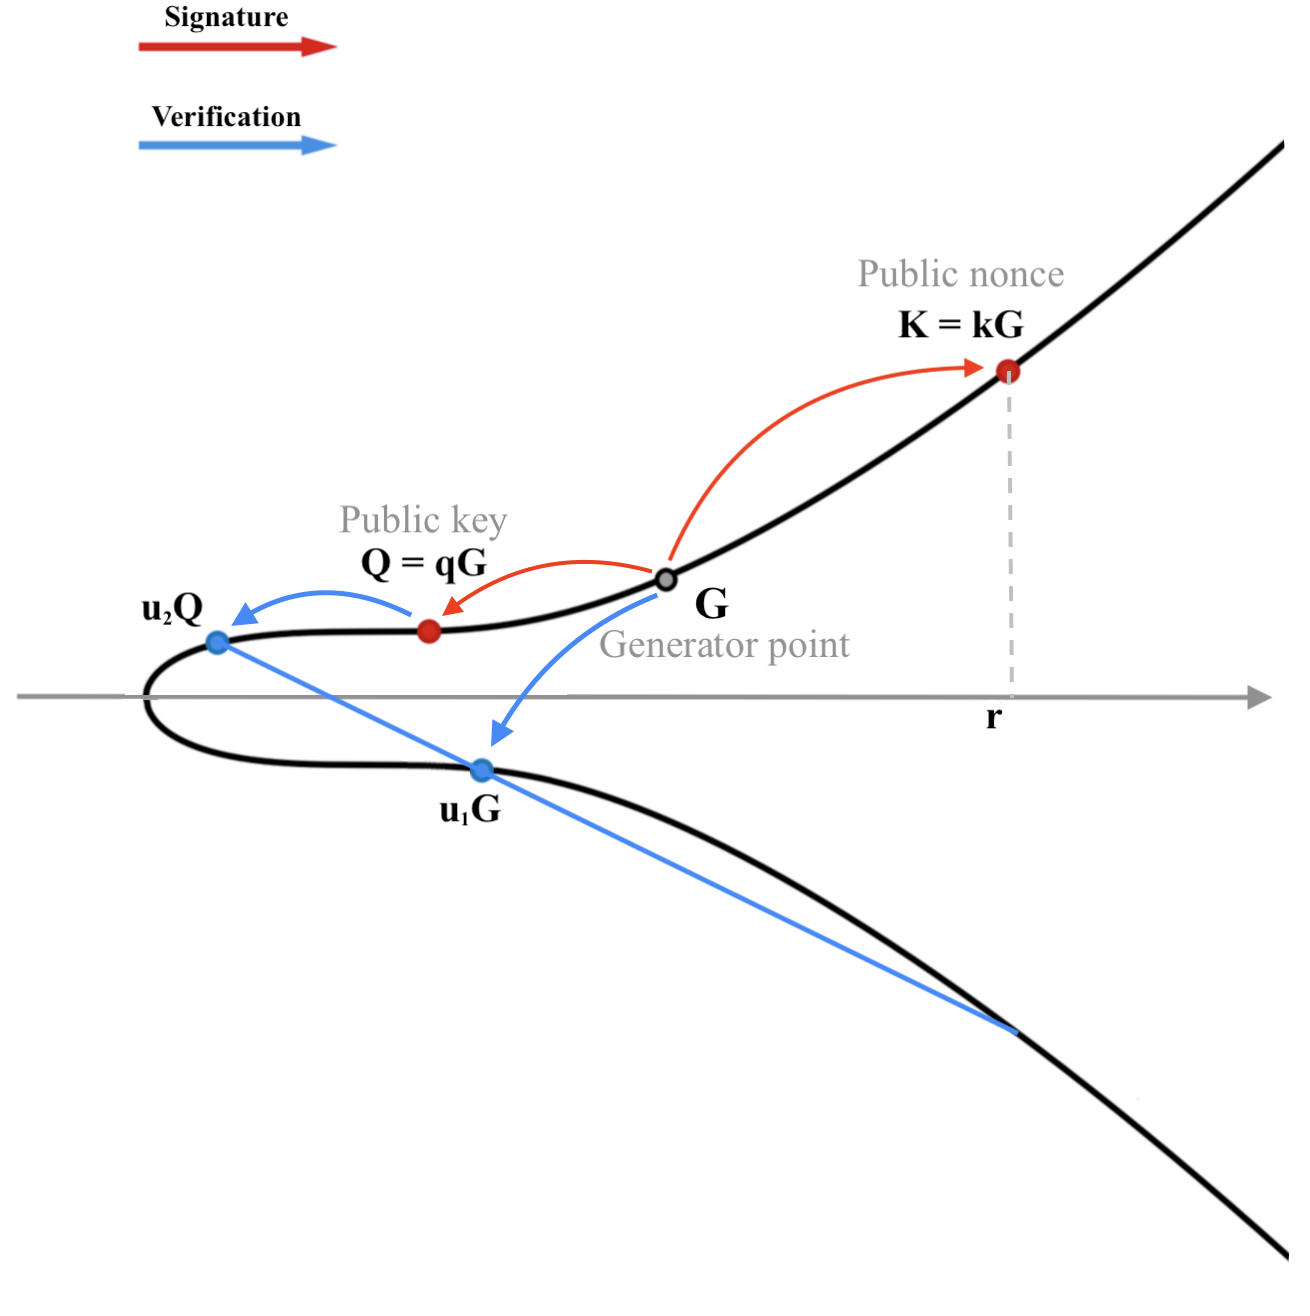
\includegraphics[scale=0.29]{images/ECDSA6}
						\source{\tiny \url{https://medium.com/cryptoadvance/how-schnorr-signatures-may-improve-bitcoin-91655bcb4744}}}
					\only<7-8> {\vspace*{-0.7cm}
						\hspace*{-1.7cm}
						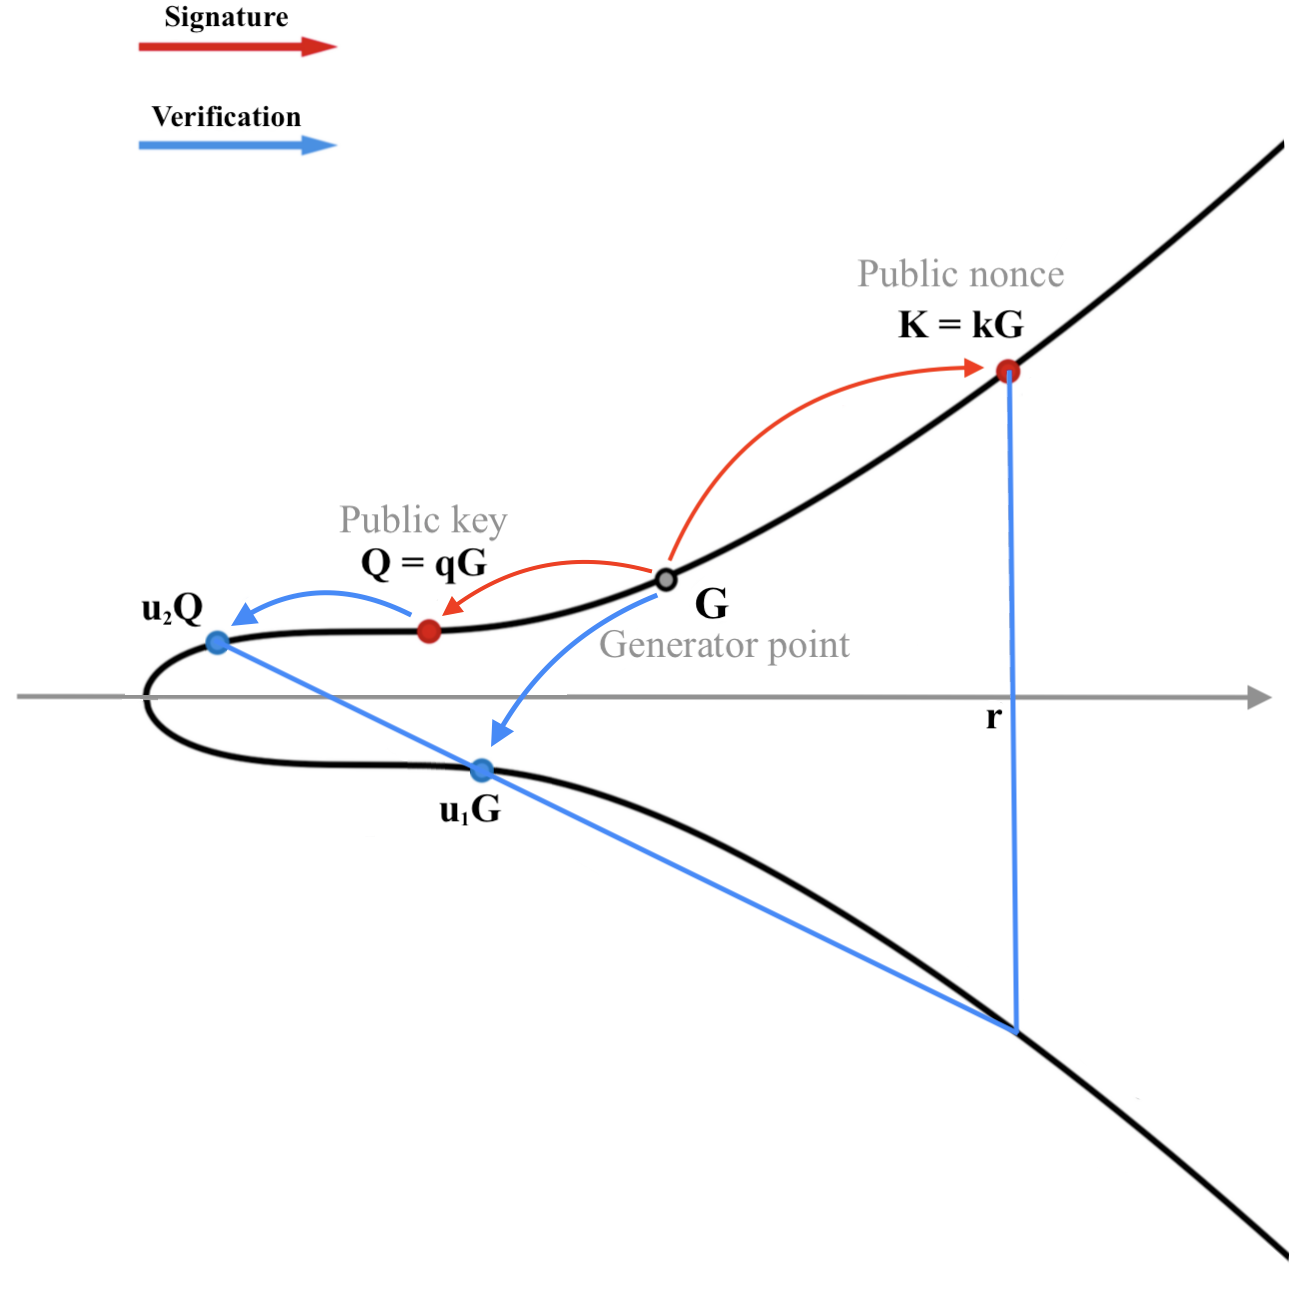
\includegraphics[scale=0.29]{images/ECDSA7}
						\source{\tiny \url{https://medium.com/cryptoadvance/how-schnorr-signatures-may-improve-bitcoin-91655bcb4744}}}
				\end{figure}
			\end{column}
		\end{columns}
	\end{frame}
	
	\subsection{ECSSA}
	\begin{frame}{Elliptic curve Schnorr signature algorithm}
		\begin{columns}
			\begin{column}{0.6\linewidth}
				ECSSA\_SIG$(m, q)$:
				\begin{enumerate}
					\item<3 -> $k \xleftarrow{\text{\$}} \{1, ..., n - 1\}$;
					\item<4 -> $K \gets kG$;
					\item<5 -> \textbf{If} $\text{jacobi}(y_K) \neq 1$: \\$\ \ \ k \gets n - k$;
					\item<6 -> $e \gets \text{hash}(x_K || qG || m) \ (\text{mod} \ n)$;
					\item<7 -> $s \gets k + eq \ (\text{mod} \ n)$;
					\item<8 -> \textbf{return} $(x_K, s)$.
				\end{enumerate}
			\end{column}
			\begin{column}{0.5\linewidth}
				\begin{figure}
					\only<1> {\vspace*{-0.7cm}
						\hspace*{-0.9cm}
						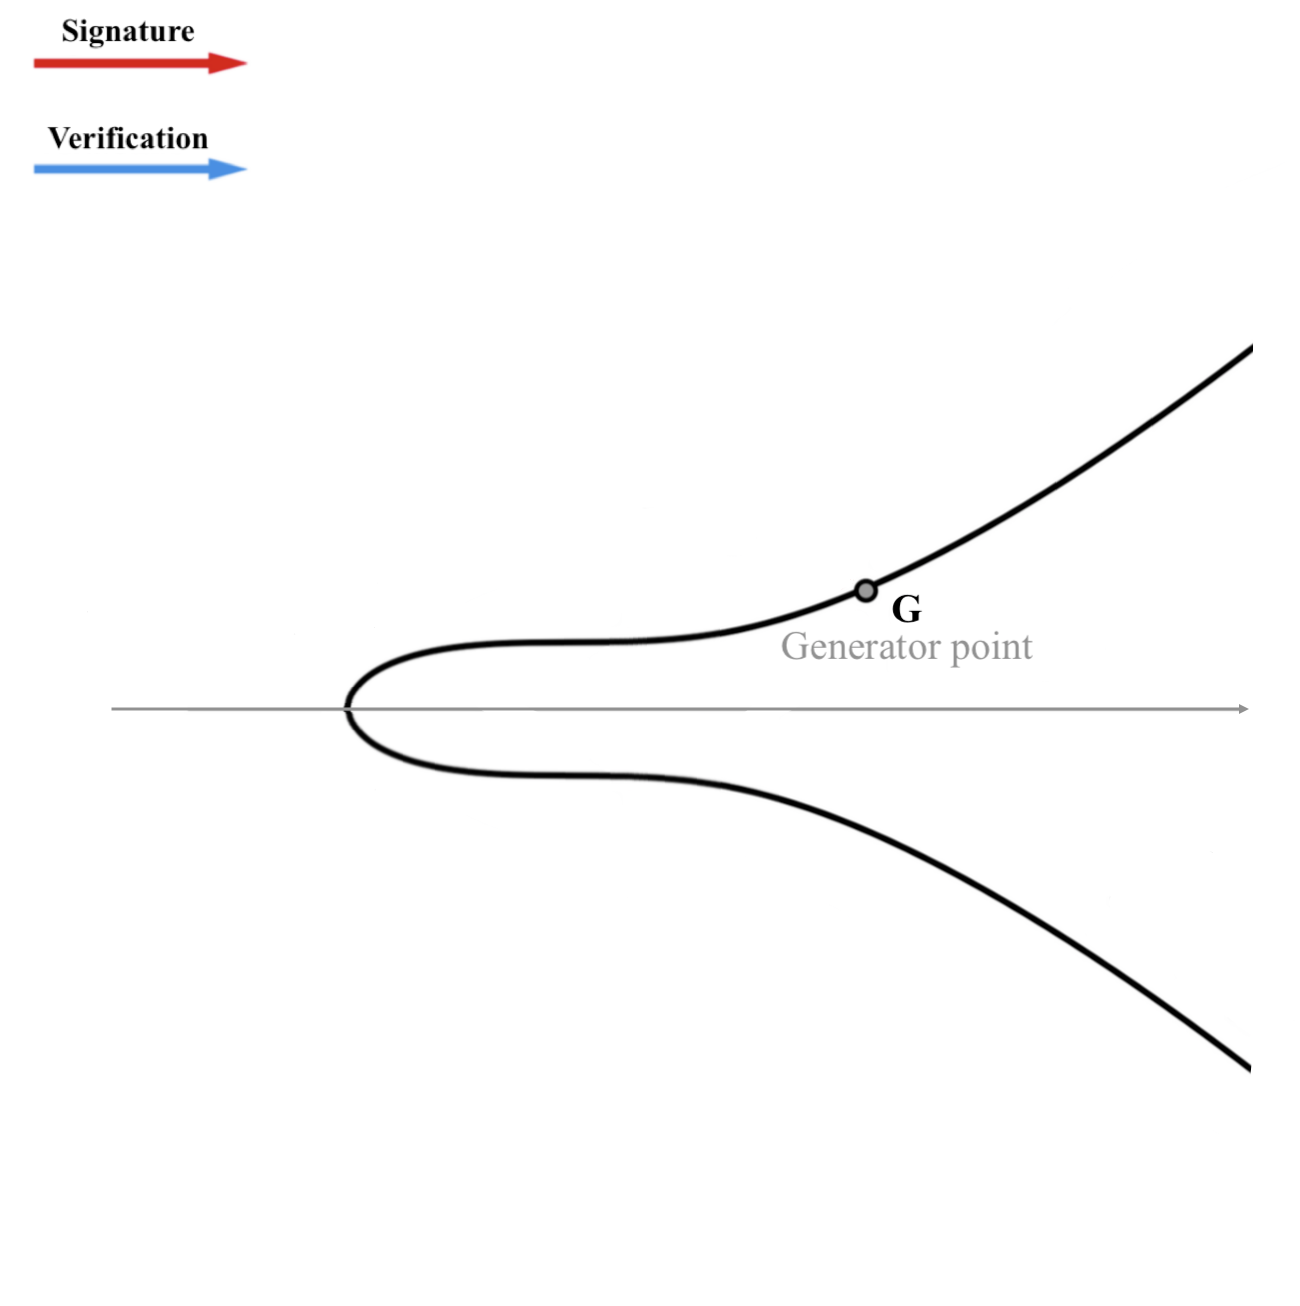
\includegraphics[scale=0.28]{images/Schnorr1}
						\source{\tiny \url{https://medium.com/cryptoadvance/how-schnorr-signatures-may-improve-bitcoin-91655bcb4744}}}
					\only<2-3> {\vspace*{-0.7cm}
						\hspace*{-0.9cm}
						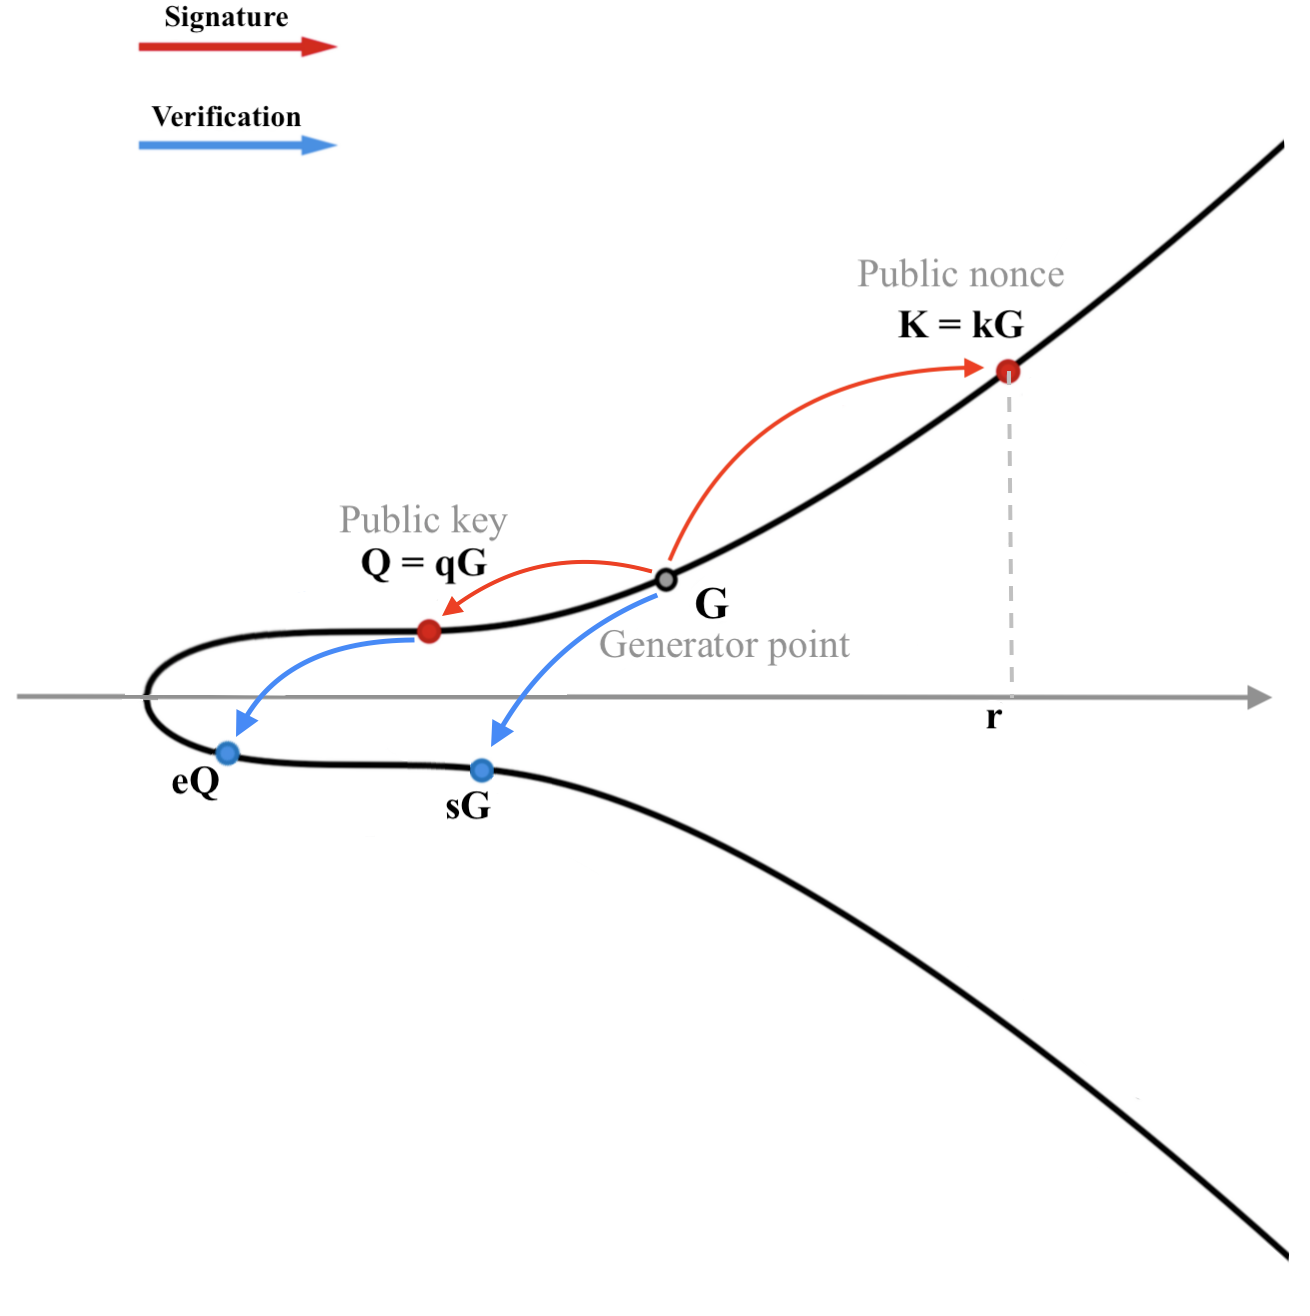
\includegraphics[scale=0.28]{images/Schnorr2}
						\source{\tiny \url{https://medium.com/cryptoadvance/how-schnorr-signatures-may-improve-bitcoin-91655bcb4744}}}
					\only<4> {\vspace*{-0.7cm}
						\hspace*{-0.9cm}
						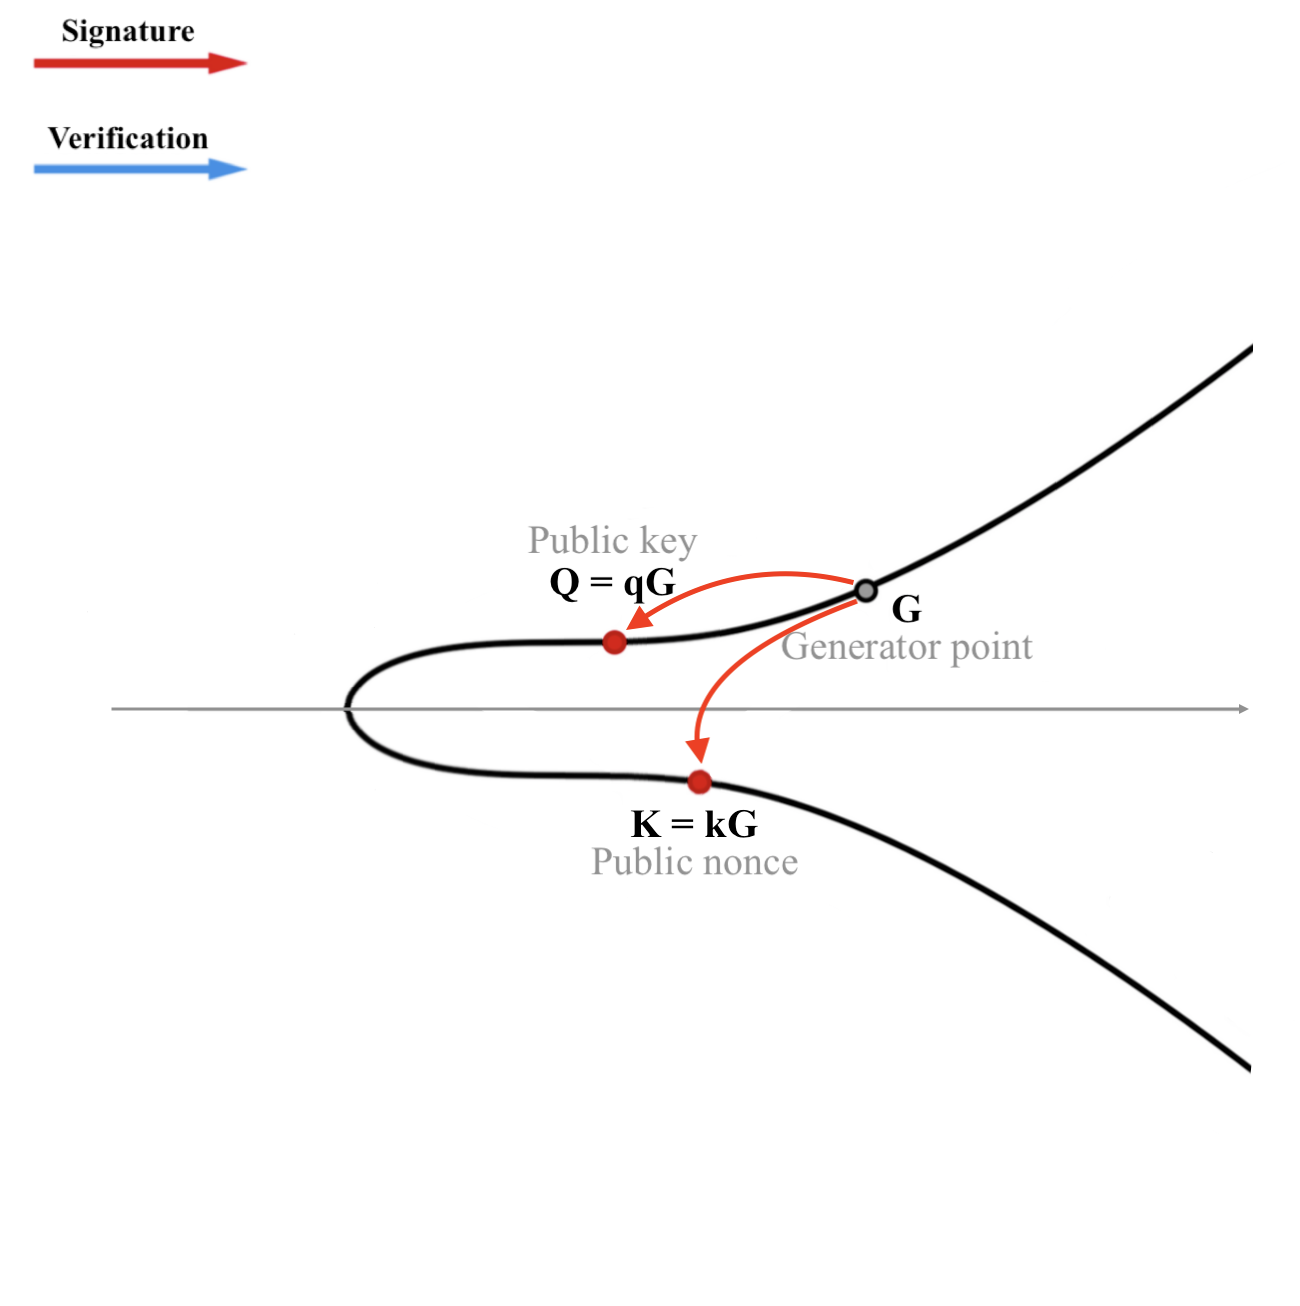
\includegraphics[scale=0.28]{images/Schnorr3}
						\source{\tiny \url{https://medium.com/cryptoadvance/how-schnorr-signatures-may-improve-bitcoin-91655bcb4744}}}
					\only<5> {\vspace*{-0.7cm}
						\hspace*{-0.9cm}
						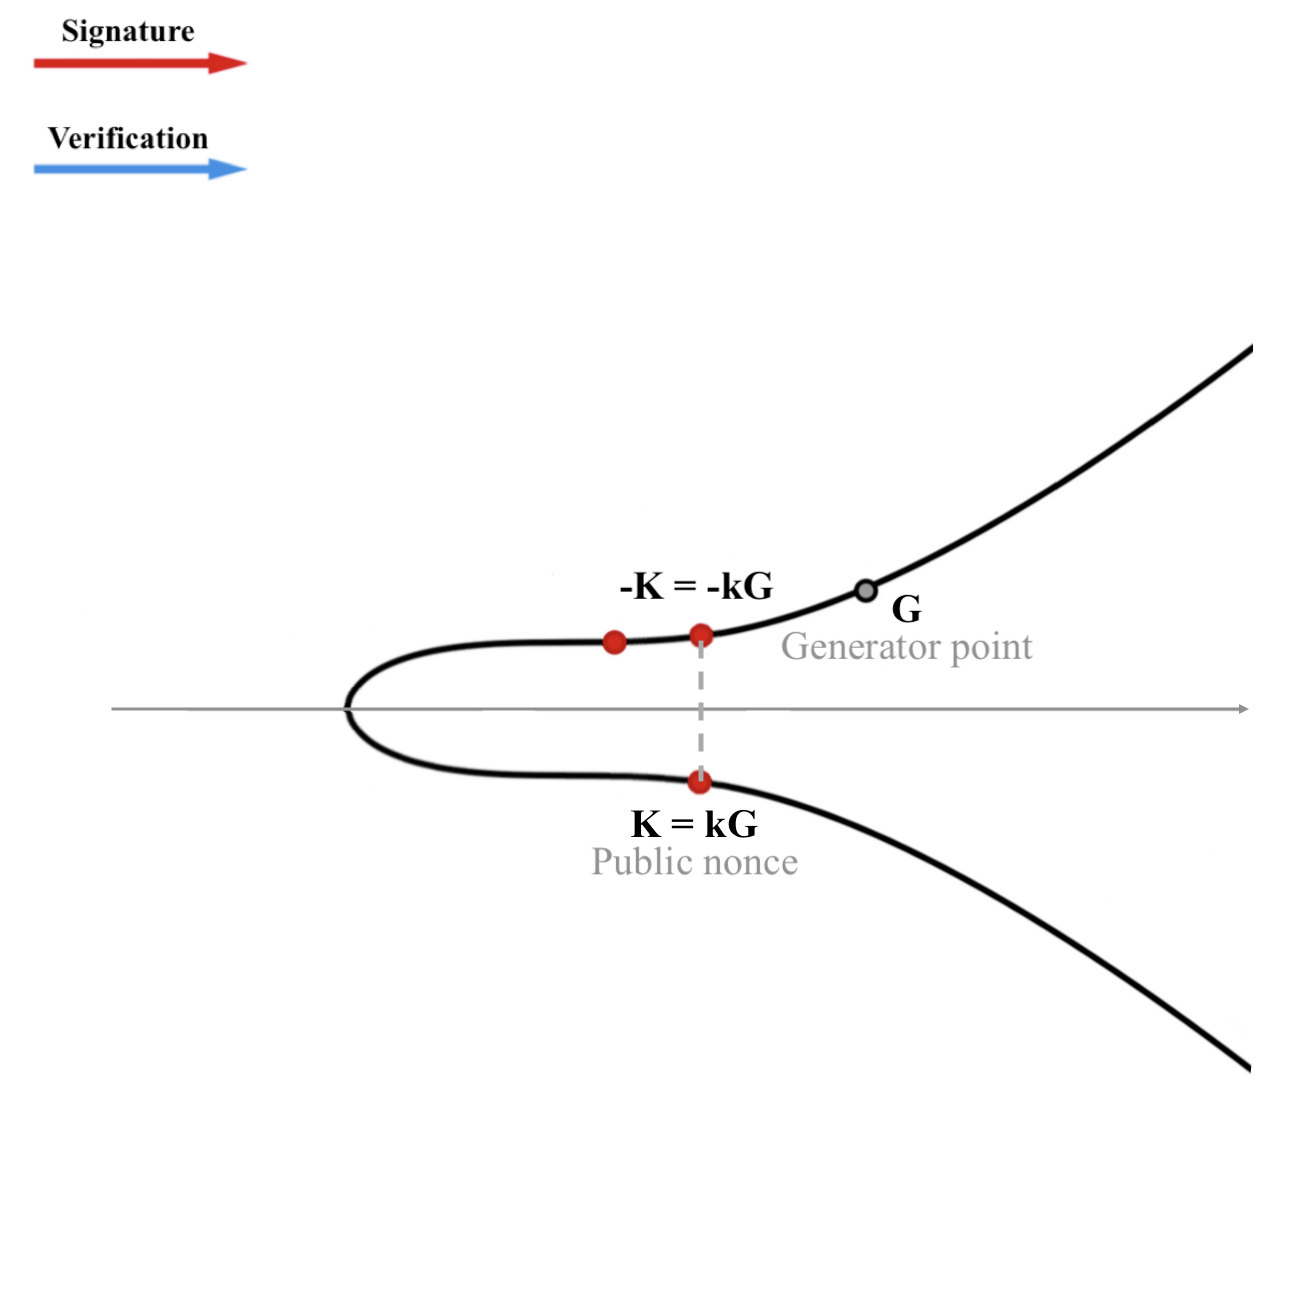
\includegraphics[scale=0.28]{images/Schnorr4}
						\source{\tiny \url{https://medium.com/cryptoadvance/how-schnorr-signatures-may-improve-bitcoin-91655bcb4744}}}
					\only<6-8> {\vspace*{-0.7cm}
						\hspace*{-0.9cm}
						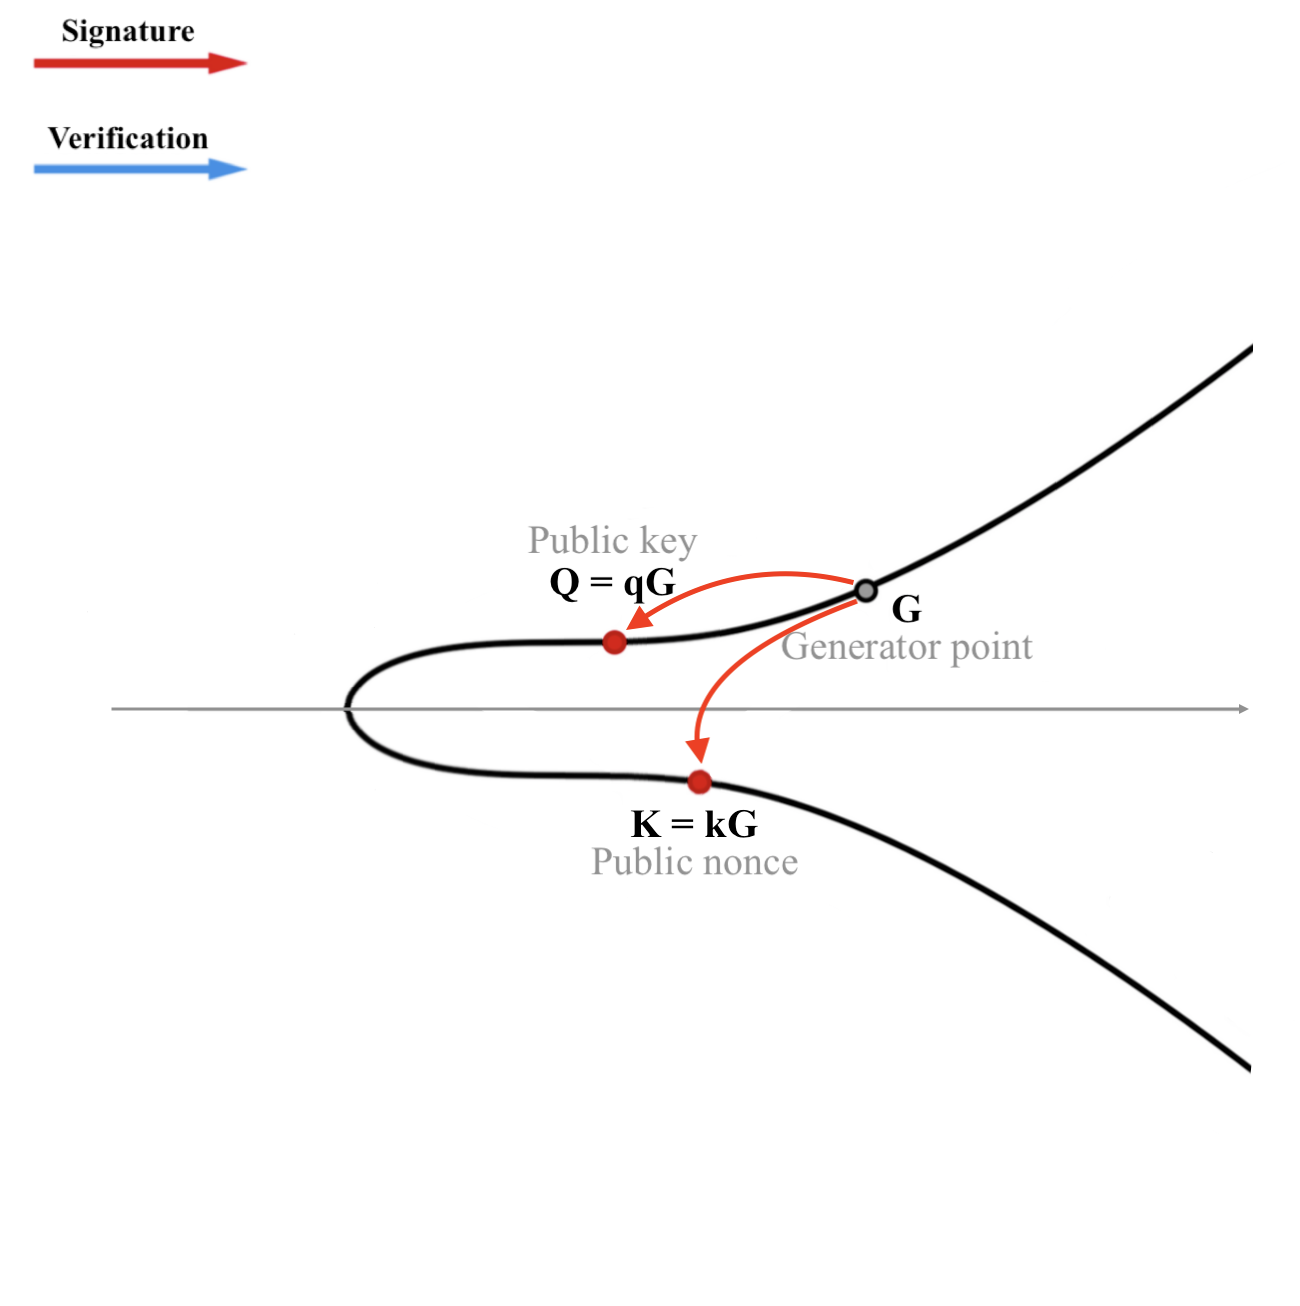
\includegraphics[scale=0.28]{images/Schnorr3}
						\source{\tiny \url{https://medium.com/cryptoadvance/how-schnorr-signatures-may-improve-bitcoin-91655bcb4744}}}
				\end{figure}
			\end{column}
		\end{columns}
	\end{frame}

	\begin{frame}{Elliptic curve Schnorr signature algorithm}
		\begin{columns}
			\begin{column}{0.6\linewidth}
				ECSSA\_VER$((r, s), m, Q)$:
				\begin{enumerate}
					\item<2 -> \textbf{If} $r \notin \{1, ..., p - 1\}$ or $s \notin \{1, ..., n - 1\}$: \\ \textbf{\ \ \ return False};
					\item<3 -> $e \gets \text{hash}(r || Q || m) \ (\text{mod} \ n)$;
					\item<4 -> $K \gets sG - eQ$;
					\item<8 -> \textbf{If} $\text{jacobi}(y_K) \neq 1$ \textbf{or} $x_K \neq r$: \\ \textbf{\ \ \ return False};
					\item<9 -> \textbf{return True}.
				\end{enumerate}
			\end{column}
			\begin{column}{0.5\linewidth}
				\begin{figure}
					\only<1-3> {\vspace*{-0.7cm}
						\hspace*{-0.9cm}
						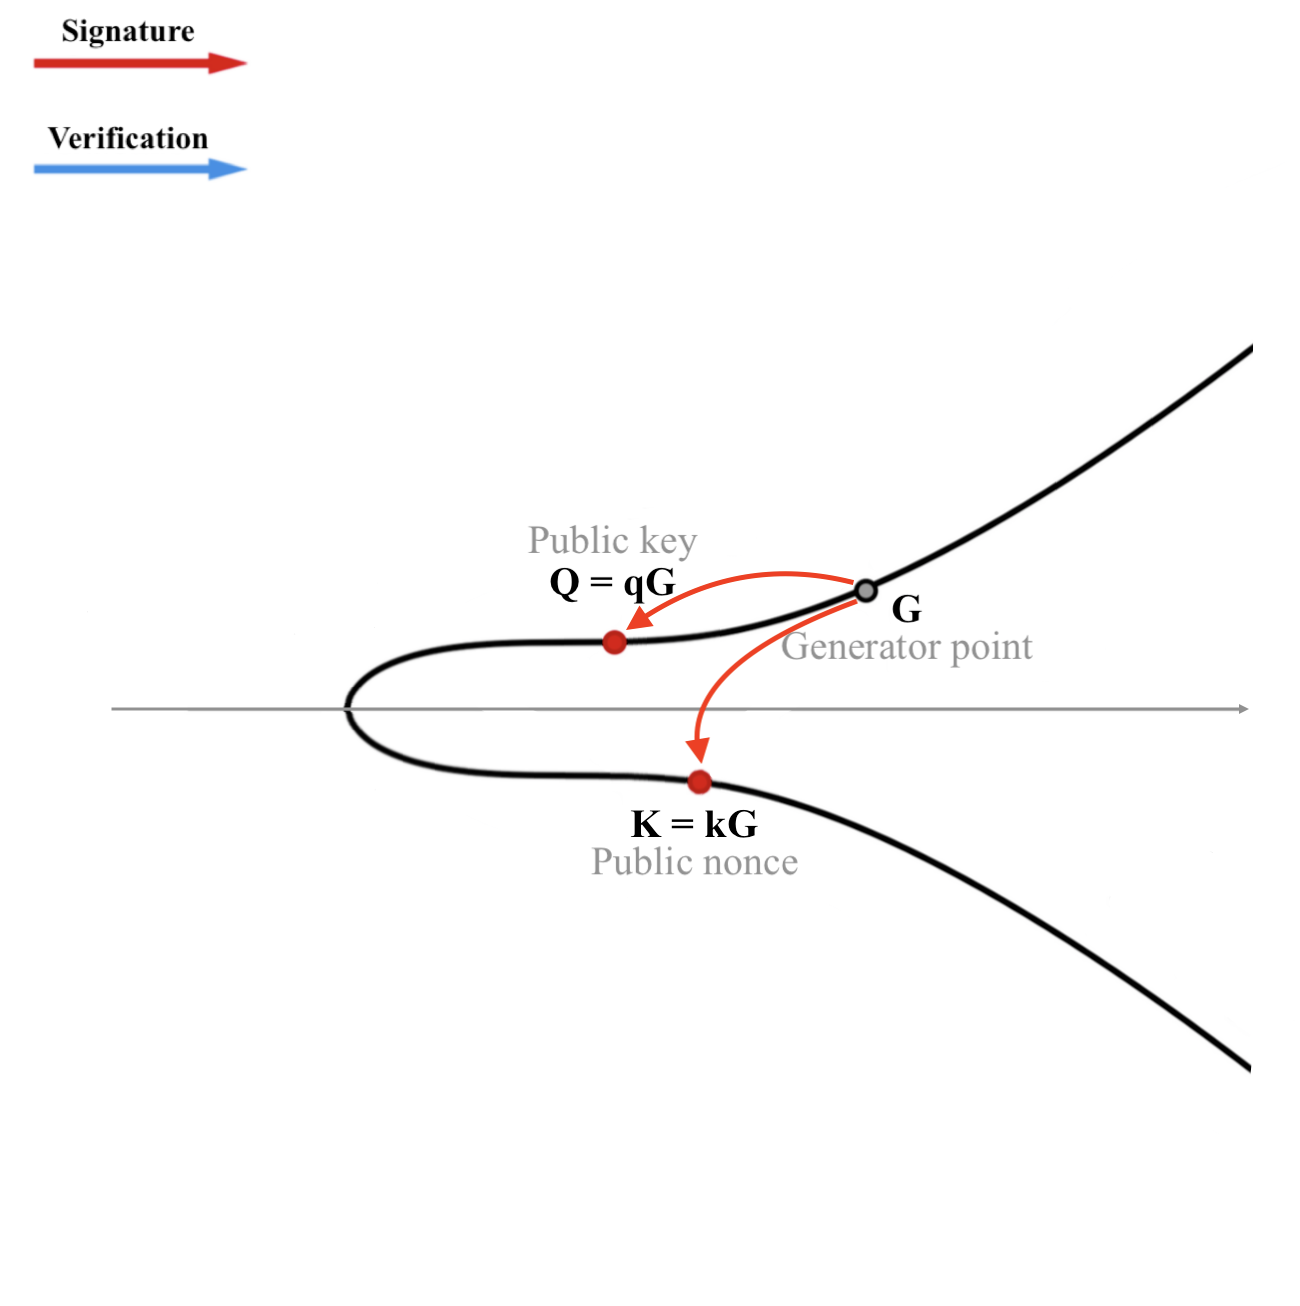
\includegraphics[scale=0.28]{images/Schnorr3}
						\source{\tiny \url{https://medium.com/cryptoadvance/how-schnorr-signatures-may-improve-bitcoin-91655bcb4744}}}
					\only<4> {\vspace*{-0.7cm}
						\hspace*{-0.9cm}
						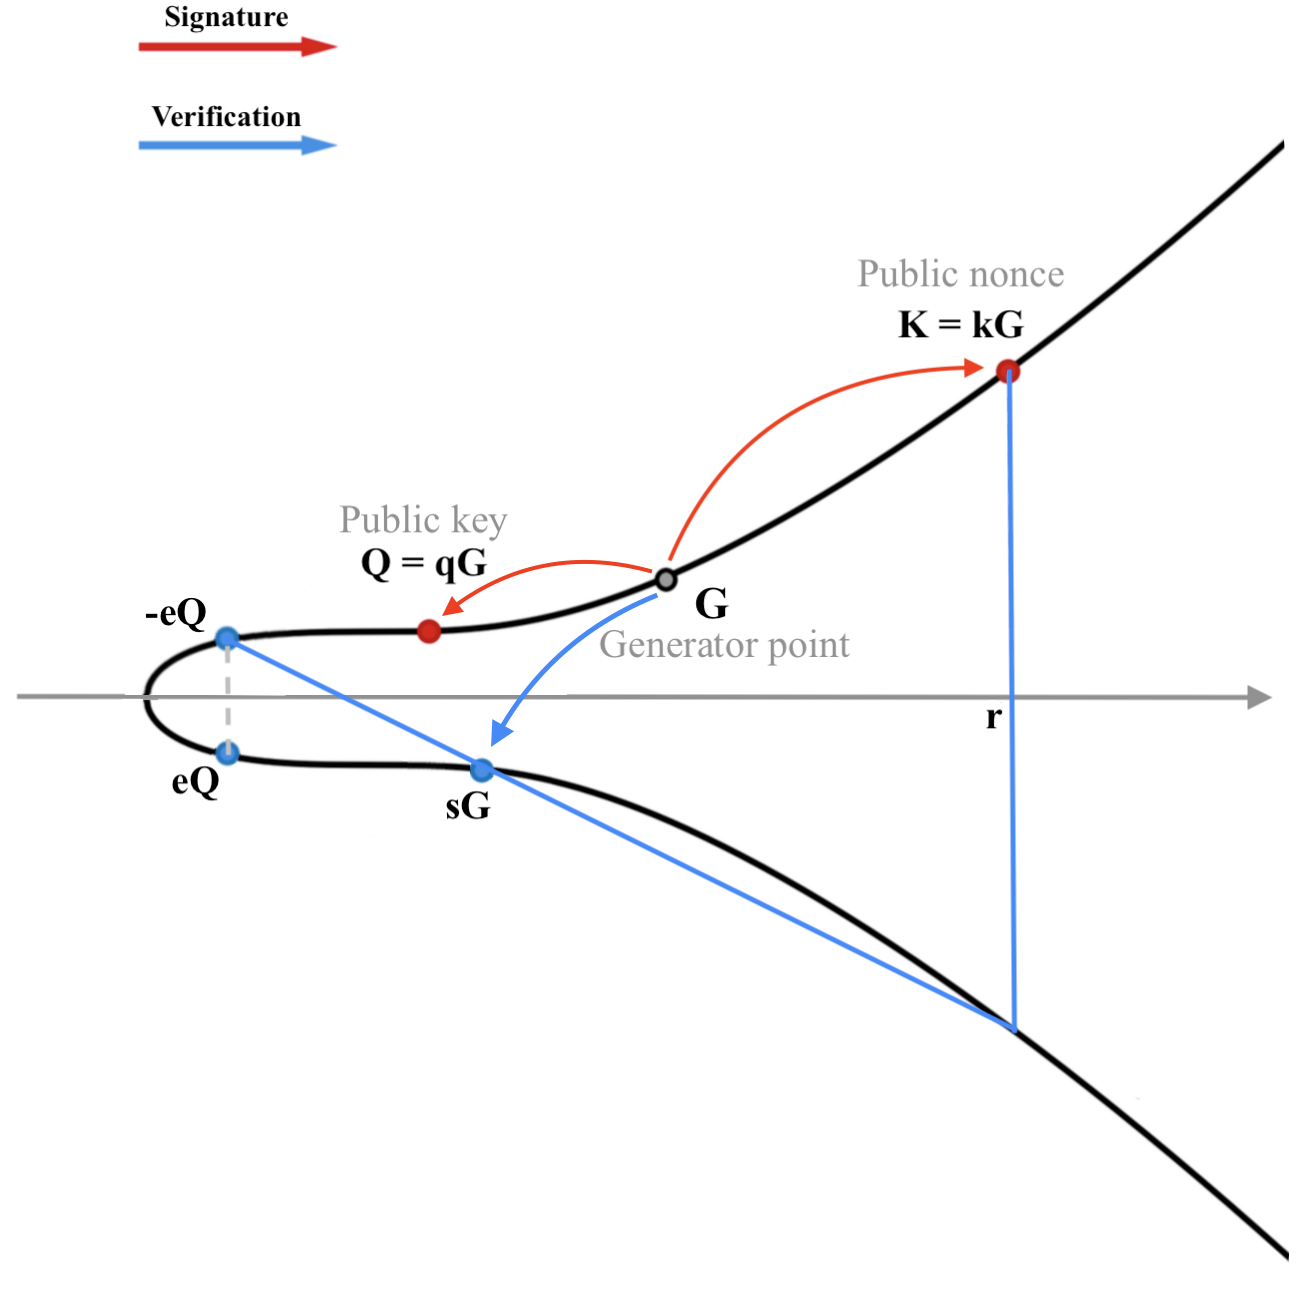
\includegraphics[scale=0.28]{images/Schnorr5}
						\source{\tiny \url{https://medium.com/cryptoadvance/how-schnorr-signatures-may-improve-bitcoin-91655bcb4744}}}
					\only<5> {\vspace*{-0.7cm}
						\hspace*{-0.9cm}
						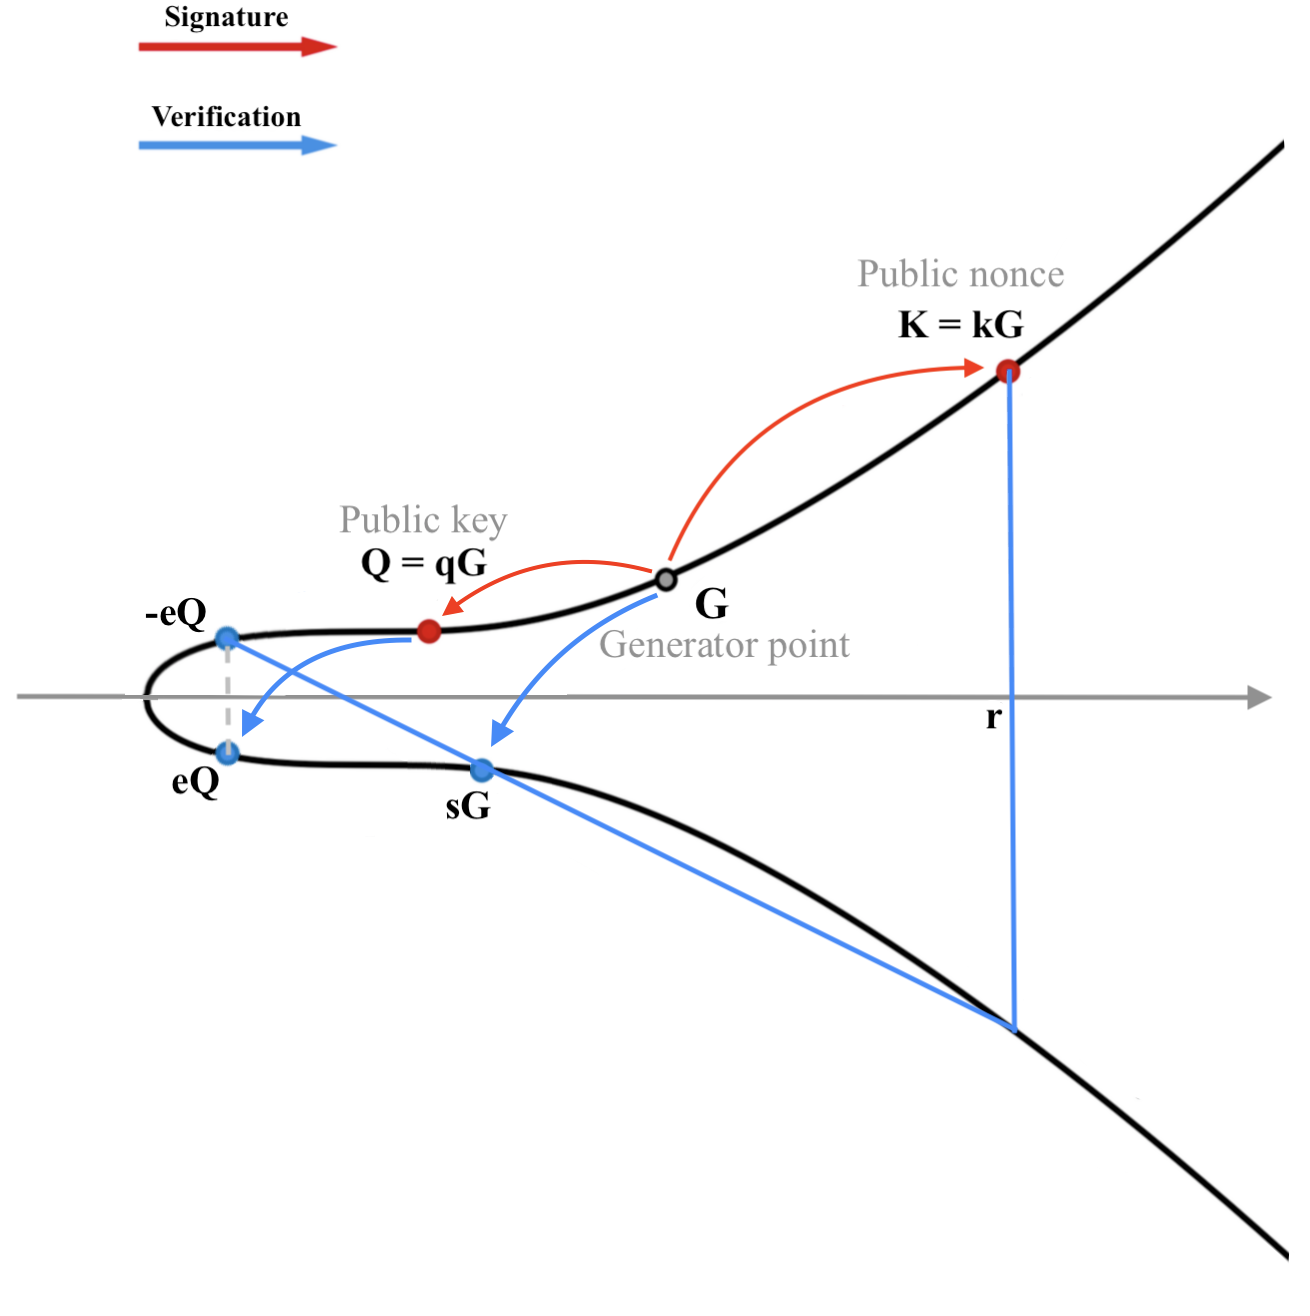
\includegraphics[scale=0.28]{images/Schnorr6}
						\source{\tiny \url{https://medium.com/cryptoadvance/how-schnorr-signatures-may-improve-bitcoin-91655bcb4744}}}
					\only<6> {\vspace*{-0.7cm}
						\hspace*{-0.9cm}
						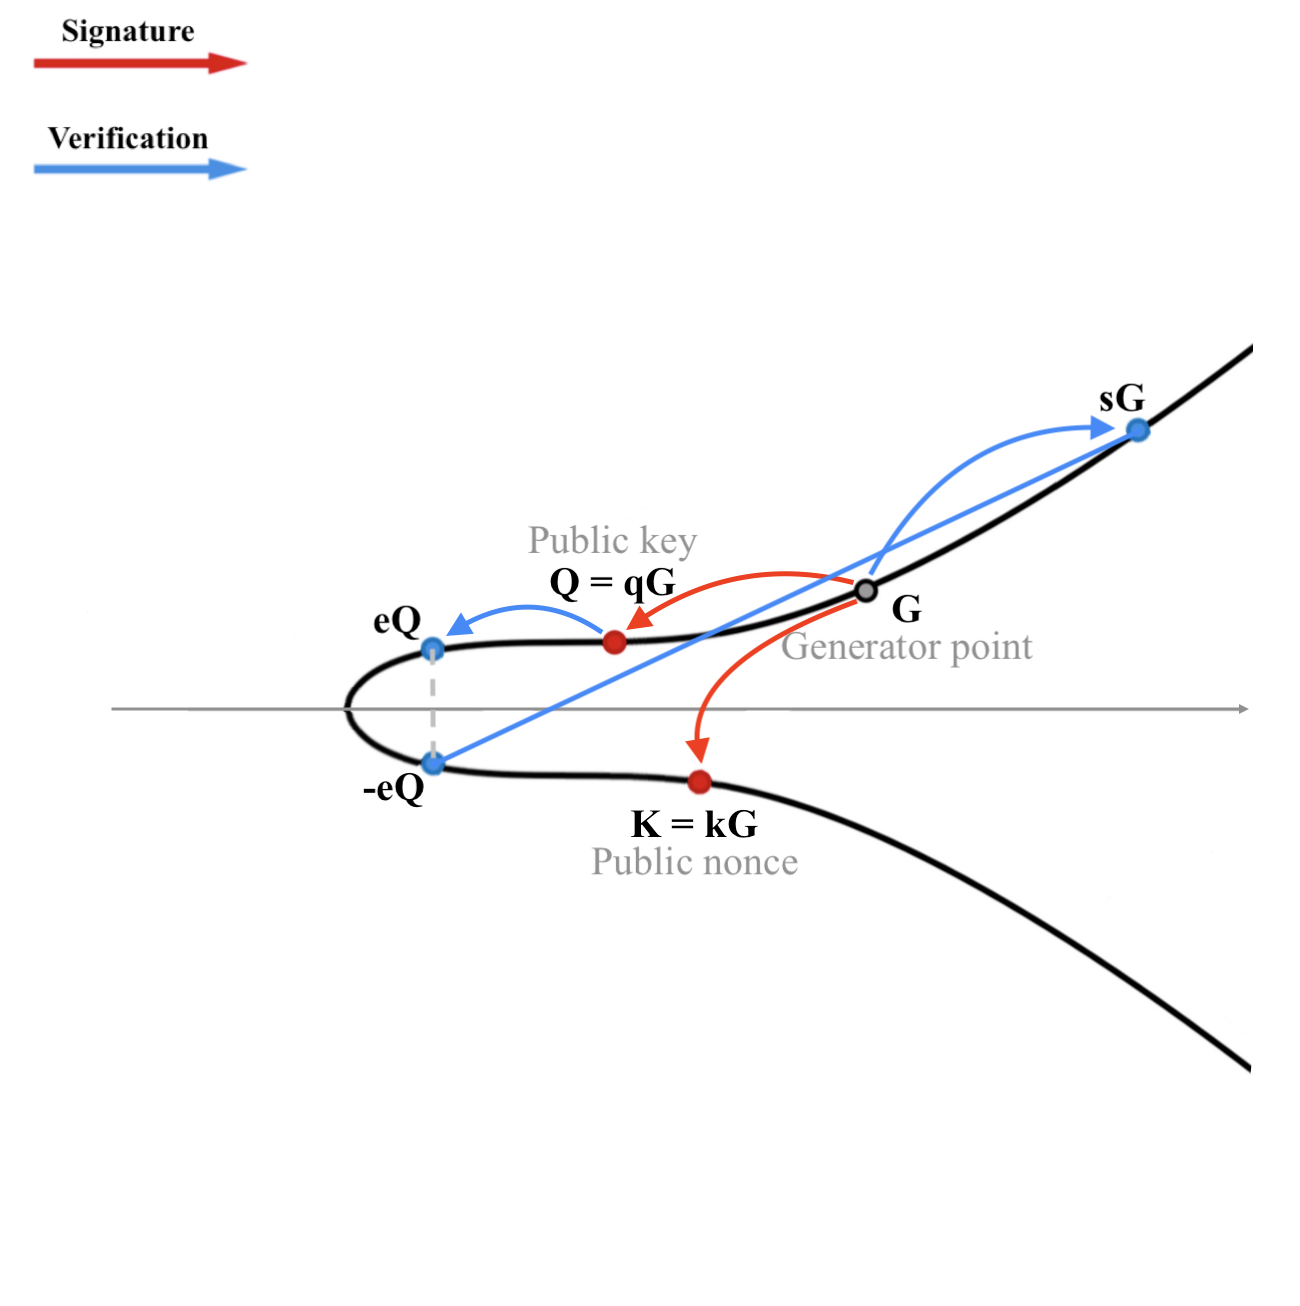
\includegraphics[scale=0.28]{images/Schnorr7}
						\source{\tiny \url{https://medium.com/cryptoadvance/how-schnorr-signatures-may-improve-bitcoin-91655bcb4744}}}
					\only<7-9> {\vspace*{-0.7cm}
						\hspace*{-0.9cm}
						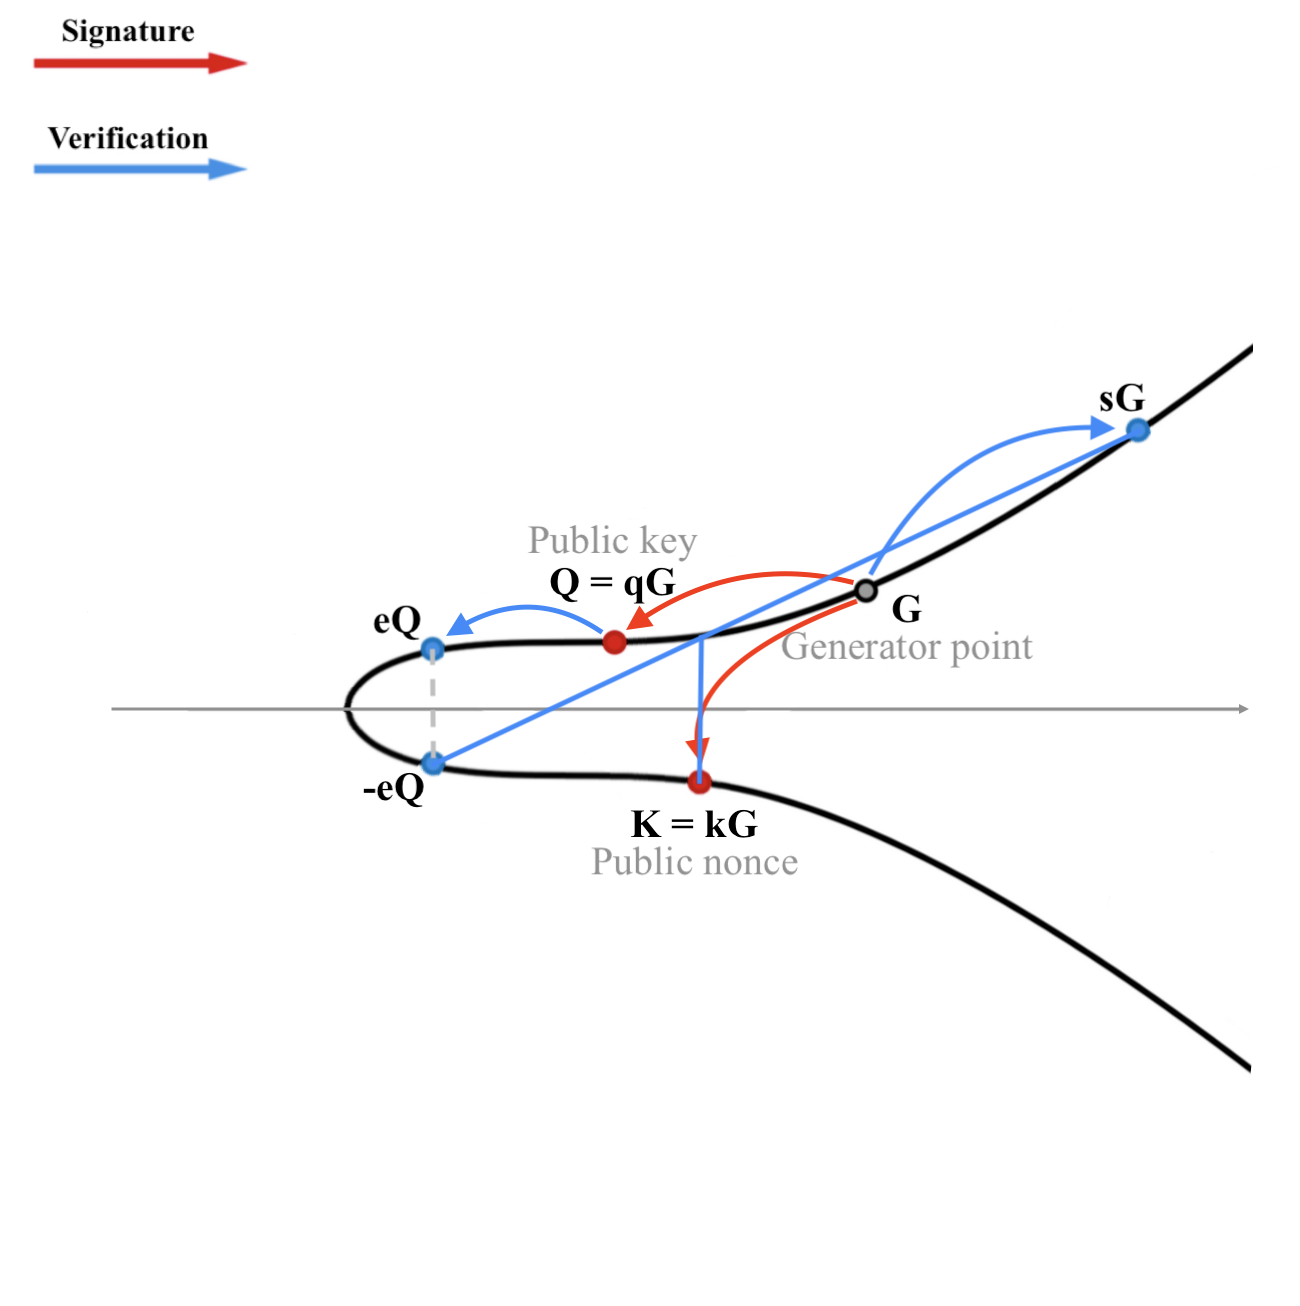
\includegraphics[scale=0.28]{images/Schnorr8}
						\source{\tiny \url{https://medium.com/cryptoadvance/how-schnorr-signatures-may-improve-bitcoin-91655bcb4744}}}
				\end{figure}
			\end{column}
		\end{columns}
	\end{frame}

	\begin{frame}{ECDSA vs. ECSSA}
		\begin{columns}
			\begin{column}{0.5\linewidth}
				ECDSA:
				\begin{itemize}
					\item<2 -> Malleable: given $(r, s)$ also $(r, -s \ (\text{mod} \ n))$ is a valid signature for same message and public key;
					\item<3 -> DER encoding: variable length, up to 73 bytes;
					\item<4 -> Chosen standardization forbid batch validation;
					\item<5 -> Requires the calculation of modular inverses;
					\item<6 -> Not linear: very complex higher level constructions.
				\end{itemize}
			\end{column}
			\begin{column}{0.5\linewidth}
				ECSSA:
				\begin{itemize}
					\item<2 -> Provably secure (SUF-CMA) in the Random Oracle Model assuming the ECDLP is hard $\Longrightarrow$ not malleable;
					\item<3 -> New encoding: fixed length, always 64 bytes;
					\item<4 -> \hyperlink{batch_validation}{Batch validation} scales logarithmically;
					\item<5 -> No computational heavy operations involved;
					\item<6 -> Linear: easier higher level constructions.
				\end{itemize}
			\end{column}
		\end{columns}
	\end{frame}
	
	\section{ECSSA applications}
	
	\subsection{Bitcoin's smart contracts}
	\begin{frame}{Bitcoin's smart contracts}
		Bitcoin has been conceived as programmable money: the funds are locked by a smart contract that settles the spending conditions.
		
		\bigskip
		\noindent
		Signatures are required to enforce property rights in the digital realm, so they are typically necessary to spend bitcoins and are embedded in the spending smma
		
		\bigskip
		\noindent
		An easy example: Pay-to-Public-Key (P2PK)
		\begin{itemize}
			\item Locking script: $<$pubKey$>$ OP\_CHECKSIG
			\item Unlocking script: $<$sig$>$
		\end{itemize}
	\end{frame}
	
	\subsection{MuSig}
	\begin{frame}{Multi-signature schemes}
		Multi-signature schemes allow a group of users to cooperate to sign a single message: they are fundamental in real life applications.
		
		\bigskip
		\noindent
		Bitcoin multi-signature ($t$-of-$m$) is implemented naively:
		\begin{itemize}
			\item Locking script: t $<$pubKey1$>$ $<$pubKey2$>$ ... $<$pubKeym$>$ \hphantom{em} \hphantom{em} \hphantom{em} \hphantom{ipsem}m
			OP\_CHECKMULTISIG
			\item Unlocking script: 0 $<$sig1$>$ $<$sig2$>$ ... $<$sigt$>$
		\end{itemize}
	
		\bigskip
		\noindent

		\onslide<2->{\alert<3>{Schnorr multi-signature (2-of-2) implemented naively:}
		\begin{itemize}
			\item\alert<3>{Alice ($\{q_A, Q_A\}$) and Bob ($\{q_B, Q_B\}$) generates $K_A$ and $K_B$;}
			\item\alert<3>{They exchange them and set the public nonce at $K = K_A + K_B$. The joint public key is set at $Q = Q_A + Q_B$;}
			\item\alert<3>{Their partial signatures are: $s_i = k_i + \text{hash}(x_K || Q || msg)q_i, \ i \in \{A, B\}$;}
			\item\alert<3>{The signature $(x_K, s_A + s_B)$ is valid on $msg$ for public key $Q$.}
		\end{itemize}}
		\onslide<3>{\huge \centering \textcolor{red}{INSECURE: rogue key attack!}}
	\end{frame}

	\begin{frame}{\hyperlink{musig}{MuSig}: compact $m$-of-$m$ signature scheme}
		To solve the problem without resorting to the Knowledge Of Secret Key (KOSK) setting, the idea is to introduce a ``random factor" (ROM) $a_i = \text{hash}(\langle L \rangle || Q_i)$ per public key $Q_i$:
		$$Q = \onslide<2->{a_1}Q_1 + \onslide<2->{a_2}Q_2 ... + \onslide<2->{a_m}Q_m.$$
		\onslide<3->{
		$$s_i = k_i + \text{hash}(x_K || Q || msg)a_iq_i \ (\text{mod} \ n), \ i = 1, ..., m.$$
		The signature $(x_K,  s =  \sum_{i = 1}^{m}s_i \ (\text{mod} \ n))$ can be verified as a simple Schnorr signature against $Q$:
		$$sG = \left(\sum_{i = 1}^{m}k_i + \text{hash}(x_K || Q || msg)\sum_{i = 1}^{m}a_iq_i\right)G  =$$
		$$= \sum_{i = 1}^{m}K_i + \text{hash}(x_K || Q || msg)\sum_{i =  1}^{m}a_iQ_i =$$
		$$= K + \text{hash}(x_K || Q || msg)Q.$$}
	\end{frame}

	\begin{frame}{\hyperlink{musig}{MuSig}: compact $m$-of-$m$ signature scheme}
		\begin{itemize}
			\item Compact: same size as the single user case;
			\item Secure in the plain public key model: allows signature aggregation at transaction level;
			\item Interactive: affects usability, prevents signature aggregation at block level;
			\item Key aggregation: signature indistinguishable from the single user case.
		\end{itemize}
		The multi-signature policy is completely hidden: this is a huge improvement for both privacy and efficiency.
	\end{frame}

	

	\subsection{Threshold signature scheme}
	\begin{frame}{\hyperlink{threshold}{Threshold signature scheme} ($t$-of-$m$)}
		\begin{itemize}
			\item Pedersen verifiable secret sharing scheme: a dealer chooses secret $r \in \{1, ..., n - 1\}$ and embeds it in a random polynomial $f(u) = r + f_1u + ... + f_{t - 1}u^{t - 1} \ (\text{mod} \ n)$. 
			\\
			Each participant $i = 1, ..., m$ of the scheme receives the share $s_i = f(i)$. To reconstruct the secret $t$ participants can rely on Lagrange's interpolation formula;
			\item Protocol for the generation of a shared random secret: every participant acts as the dealer in the previous protocol. 
			\begin{itemize}
				\item Shared secret: $r = \sum_{i = 1}^{m}r_i \ (\text{mod} \ n)$;
				\item Share of the secret belonging to $i$: $s_i = \sum_{j = 1}^{m}f_j(i) \ (\text{mod} n)$.
			\end{itemize}
		To the shared secret $r$ we can associate the random polynomial $F(u) = \sum_{i}f_i(u)$ and the public key $R = rG$.
		\end{itemize}
	\end{frame}

	\begin{frame}{\hyperlink{threshold}{Threshold signature scheme} ($t$-of-$m$)}
		The protocol for the generation of a shared random secret is run twice to establish a key pair $\{q, Q\}$ (shares $\alpha_i = F_1(i)$) and a nonce pair $\{k, K\}$ (shares $\beta_i = F_2(i)$).
		
		\bigskip
		\noindent
		Each signer computes his partial signature as $\gamma_i = \beta_i + e\alpha_i \ (\text{mod} \ n)$, $e = \text{hash}(x_K || Q || msg)$.
		
		\bigskip
		\noindent
		The signature is $(x_K, s)$, with $s = \sum_{j}\gamma_j\omega_j$, where $\omega_j = \prod_{h \neq j}\frac{h}{h - j} \ (\text{mod} \ n)$.
		$s$ computed in this way satisfies $s = k + eq \ (\text{mod} n)$: 
		$$F_3(u) = F_2(u) + eF_1(u) \ \Longrightarrow \ s := F_2(0) + eF_1(0) = k + eq \ (\text{mod} \ n).$$
		$$F_3(i) = F_2(i) + eF_1(i) = \beta_i + e\alpha_i \ (\text{mod} \ n).$$
	\end{frame}

	\begin{frame}{ECDSA vs. ECSSA (multi-signature)}
		ECDSA:
		\begin{itemize}
			\item Locking script: t $<$pubKey1$>$ $<$pubKey2$>$ ... $<$pubKeym$>$ \hphantom{em} \hphantom{em} \hphantom{em} \hphantom{ipsem}m
			OP\_CHECKMULTISIG
			\item Unlocking script: 0 $<$sig1$>$ $<$sig2$>$ ... $<$sigt$>$
		\end{itemize}
		
		$\Longrightarrow$ 33 bytes * $m$ + 70 bytes * $t$. 
		
		\bigskip
		\noindent
		ECSSA:
		\begin{itemize}
			\item Locking script: $<$jointPubKey$>$ OP\_SCHNORR
			\item Unlocking script: $<$jointSig$>$
		\end{itemize}
	
	 $\Longrightarrow$ 33 bytes + 64 bytes.
	 
	 Una media sugli ultimi due anni: 1800 tx. per blocco, 500 bytes per transazione.
	\end{frame}

	\subsection{Adaptor signatures}
	\begin{frame}{Adaptor signatures}
		Building block for \textit{scriptless script}: aim at encapsulating the flexibility of script semantics in fixed size signatures.
		
		\bigskip
		\noindent
		The idea is to add to the public nonce $K$ a random $T = tG$ (public adaptor) but still consider $k$ as private nonce: this results in an invalid signature, however learning $t$ (private adaptor) is equivalent to learn a valid signature:
		$$(x_T, x_{K + T}, \tilde{s}), \ \tilde{s} = k + \text{hash}(x_{K + T}||Q||m).$$
		{\centering
		Checking equation: $\tilde{s}G = K + \text{hash}(x_{K + T}||Q||m)Q.$
		\par}
		
		\bigskip
		\noindent
		Adaptor signatures can be used in conjunction with the MuSig protocol:
		a signer generates $s_i' = k_i + \text{hash}(x_K || Q || msg)a_iq_i + t \ (\text{mod} \ n)$ after having used $K_i + T$ as public nonce.
	\end{frame}

	\begin{frame}{Cross-chain atomic swaps}
		Exchange of different crypto-currencies among two distrustful users in an atomic and decentralized way.
		
		\bigskip
		\noindent
		Nowadays, this is done via Hashed TimeLock Contract (HTLC), special locking scripts that ensures the atomicity of the transactions on both blockchains:
		\begin{itemize}
			\item Locking script: \\
			\ \ OP\_IF
			\\
			\ \ \ \ \ \ \ OP\_HASH256 $<$digest$>$ OP\_EQUALVERIFY OP\_DUP \\ 
			\ \ \ \ \ \ \ OP\_HASH160 $<$Bob address$>$ \\
			\ \ OP\_ELSE \\
			\ \ \ \ \ \ \ $<$num$>$ OP\_CHECKSEQUENCEVERIFY OP\_DROP \\ 
			\ \ \ \ \ \ \ OP\_DUP OP\_HASH160 $<$Alice address$>$ \\
			\ \ OP\_ENDIF \\
			\ \ OP\_EQUALVERIFY OP\_CHECKSIG
			\item Unlocking script:
			\begin{itemize}
				\item $<$Bob sig$>$ $<$Bob pubkey$>$ $<$preimage$>$ 1
				\item $<$Alice sig$>$ $<$Alice pubkey$>$ 0
			\end{itemize}
		\end{itemize}
	\end{frame}

	\begin{frame}{\hyperlink{atomic_swap}{Cross-chain atomic swaps via adaptor signature}}
		\begin{itemize}
			\item Alice and Bob agree on a pair of transactions which are secured by the pairs of keys ($Q^A_1$ , $Q^B_1$) and ($Q^A_2$ , $Q^B_2$), aggregated through the MuSig protocol;
			\item They engage the MuSig protocol to spend from the two transactions, but Bob generates in parallel adaptor signatures for both transactions: Alice has to verify them, in particular she needs to ensure that he used the same $t$ value;
			\item This results in two invalid signatures: but Bob, knowing $t$, can build the a corresponding valid signature;
			\item When he finally takes Alice's coins, he publish this valid signature on chain: Alice, that has to monitor the blockchain, learns it. But since she has the corresponding adaptor signature she can extract $t$ and take Bob's coins.
		\end{itemize}
	\end{frame}

	\begin{frame}{Cross-chain atomic swaps via adaptor signature}
		Efficiency and privacy gains:
		\begin{itemize}
			\item We were able to condensate the verbose script semantics of the HTLC in a signature;
			\item The policy is indistinguishable from the single user setting (adaptor signatures are deniable: for every signature on the blockchain one can come up with some $t$ and construct an adaptor signature);
			\item It is impossible to link the two transactions.
		\end{itemize}
	\end{frame}

	\section{Conclusion}
	\begin{frame}{Conclusion}
		We have seen that Schnorr would result in huge privacy (fungibility) and efficiency (scalability) improvements for Bitcoin:
		\begin{itemize}
			\item  Batch validation: a group of signatures could be validated much faster;
			\item Smaller key size, aggregation at transaction level, reduction of scripts to signatures: smaller blockchain and hidden policies;
			\item Improved security, being Schnorr signature provably secure;
		\end{itemize}
	
	\onslide<2->{But there is even more:
		\begin{itemize}
			\item Adaptor signatures could be applied also to layer 2 protocols (e.g. Lightning Network) with huge enhancements in privacy;
			\item Taproot: built on top of the concepts of Merkelized Abstract Syntax Tree (MAST) and Pay-To-Contract its aim is to make any arbitrary script, no matter how complex it is, to look the same as a single signer transaction in the cooperative case.
		\end{itemize}}
	\end{frame}

	\begin{frame}
		\centering
		\huge Thank you for your attention!
		\par
	\end{frame}
	
	\begin{frame}[t, allowframebreaks]
	\frametitle{References}
    	\setbeamertemplate{bibliography item}[text]
    	\bibliographystyle{plain}
		\nocite{*}
		\bibliography{biblio}
	\end{frame}
	
	\appendix
	\backupbegin
	\begin{frame}[label=point_addition]{Point addition - Geometric interpretation}
		\begin{columns}
			\begin{column}{0.5\linewidth}
				The intuition to add points belonging to an EC defined over a finite field is the same presented for the curve defined over the real numbers: draw the line passing through the points (that repeats along the plane in this case) until it intersects a third point: then reflect this point with respect to the line $y = \frac{p}{2}$, i.e. apply the transformation $(x_3, y_3) \to (x_3, p - y_3)$.
			\end{column}
			\begin{column}{0.6\linewidth}
				\begin{tikzpicture}[
				every node/.style = {% is not necessary, default node's shape is rectangle
					align=center}
				]
				
				\node () at (0,0) {};
				\node (a) {\includegraphics[height=5cm, width=6.6cm]{images/sum_ec_over_ff}};
				
				\node (b) [below=of a, yshift = 1.2cm] {\small The curve $y^2 = x^3 - x + 3 \ \text{over} \ \mathbb{F}_{127}$.};
				\end{tikzpicture}
			\end{column}
		\end{columns}
	\end{frame}

	\begin{frame}{Point addition - Algebraic formulas}
		There are some cases to be considered:
		\begin{itemize}
			\item $Q_2 = -Q_1$: by definition we have $Q_1 + Q_2 = \infty$, where $\infty$ is the identity element of the addition operation;
			\item $Q_2 = \infty$: $Q_1 + Q_2 = Q_1$;
			\item $Q_2 = Q_1$: $x_3 = m^2 - 2x_1$ and $y_3 = m(x_1 - x_3) - y_1$, where $m = \frac{3x_1^2 + a}{2y_1}$;
			\item $Q_2 \neq \pm Q_1$: $x_3 = m^2 - x_1 - x_2$ and $y_3 = m(x_1 - x_3) - y_1$, where $m = \frac{y_2 - y_1}{x_2 - x_1}$.
		\end{itemize}
	\end{frame}
	
	\begin{frame}[label = double_add]{Double and add algorithm}
		Scalar multiplication is the core of ECC due to its computational asymmetry:
		\begin{itemize}
			\item The direct operation $q \to Q$ can be made efficiently (i.e. there exist some polynomial time algorithms);
			\item The inverse operation $Q \to q$ in general cannot be made efficiently (i.e. do not exist sub-exponential algorithms).
		\end{itemize}
	
		\bigskip
		\noindent
			
		\begin{block}{Double and add algorithm: $q = 41$}
			We decompose $q$ according to its binary representation:
			$$41 = 1 + 8 + 32  \ \Longrightarrow \ 41G = G + 8G + 32G.$$
			
			\noindent
			5 point doubling and 2 additions vs. 40 additions.
	\end{block}
	\end{frame}

	\begin{frame}[label = batch_validation]{Batch validation}
		A signature $(K, s)$ is valid if $K = sG - \text{hash}(x_K \ || \ Q \ || \ m)Q$. Thus, two valid signatures $(K_0, s_0)$ and $(K_1, s_1)$ satisfies:
		$$K_0 + K_1 = (s_0 + s_1)G - \text{hash}(x_{K_0} \ || \ Q_0 \ || \ m_0)Q_0 - \text{hash}(x_{K_1} \ || \ Q_1 \ || \ m_1)Q_1.$$
		Insecure: introduction of random factors.
		$$a_0K_0 + a_1K_1 =$$ $$
		= (a_0s_0 + a_1s_1)G - a_0\text{hash}(x_{K_0} \ || \ Q_0 \ || \ m_0)Q_0 - a_1\text{hash}(x_{K_1} \ || \ Q_1 \ || \ m_1)Q_1.$$
	\end{frame}

	\begin{frame}{Batch validation - Bos-Coster's algorithm}
		\begin{columns}
			\begin{column}{0.5\linewidth}
				$\ \ \ \ \ \ \ \ \ \ a_0K_0 + a_1K_1 =$ \\ $= (a_0 - a_1)K_0 + a_1(K_0 + K_1)$.
				
				\bigskip
				
				\begin{itemize}
					\item Sort the tuples according to $a_i$ in descending order;
					\item While the list has length larger than one:
					\begin{itemize}
						\item Substitute $(a_0, K_0)$ and $(a_1, K_1)$ with $(a_0 - a_1, K_0)$ and $(a_1, K_0 + K_1)$;
						\item Sort the list again;
					\end{itemize}
					\item When only one element remains, with very large probability it will be of the form $(1, K)$, otherwise it will be of the form $(a, K)$.
				\end{itemize}
			\end{column}
			\begin{column}{0.5\linewidth}
				\hspace*{0cm}
				\includegraphics[scale=0.3]{images/speedup}
			\end{column}
		\end{columns}
	\end{frame}

	\begin{frame}[label = musig]{MuSig: compact $m$-of-$m$ signature scheme}
	\begin{columns}
		\begin{column}{0.5\linewidth}
			\only<1-18>{
				MuSig($m, q_1, \langle L \rangle$):
				\begin{enumerate}
					\item<2 -> \textbf{for} $i \gets 1, m$ \textbf{do}:
					\begin{enumerate}
						\item<2 -> $a_i \gets \text{hash}(\langle L\rangle || Q_i)$;
					\end{enumerate}
					\item<3 -> $Q \gets \sum_{i = 1}^{m} a_iQ_i$;
					\item<4 -> $k_1 \xleftarrow{\text{\$}} \{1, ..., n - 1\}$;
					\item<5 -> $K_1 \gets k_1G, \ t_1 \gets \text{hash}(K_1)$;
					\item<6 -> \textbf{send} $t_1, K_1$;
					\item<11 -> $K \gets \sum_{i = 1}^{m} K_i$;
					\item<13 -> $c \gets \text{hash}(x_K || Q || m)$;
					\item<14 -> $s_1 \gets k_1 + ca_1q_1 \ (\text{mod} \ n)$;
					\item<15 -> \textbf{send} $s_1$;
					\item<17 -> $s \gets \sum_{i = 1}^{m} s_i \ (\text{mod} \ n)$;
					\item<18 -> \textbf{return} $(x_K , s)$.
				\end{enumerate}
			}
		\end{column}
		\begin{column}{0.62\linewidth}
			\begin{center}
				\begin{tikzpicture}[
				every node/.style = {% is not necessary, default node's shape is rectangle
					align=center}
				]
				
				
				\onslide<1-> {\node (a) {\includegraphics[scale=0.17]{images/Alice.jpg}};}
				\onslide<1-> {\node (b) [text width=3cm, below=of a, yshift=1cm] {1: Alice};}
				
				\onslide<1-> {\node (d) [right=of a] {\includegraphics[scale=0.22]{images/Bob.jpg}};}
				\onslide<1-> {\node (e) [text width=3cm, below=of d, yshift=1cm] {2: Bob};}
				
				\onslide<1-> {\node (g) [below=of a, xshift=2cm] {\includegraphics[scale=0.1717]{images/Charlotte.jpg}};}
				\onslide<1-> {\node (h) [text width=3cm, below=of g, yshift=1cm] {3: Charlotte};}
				
				\only<2>{\node (i) [right=of a, xshift=-1.5cm, yshift=0.5cm] {$a_1, a_2, a_3$}};
				\only<3>{\node (i) [right=of a, xshift=-1.5cm, yshift=0.5cm] {$Q$}};
				\only<4>{\node (i) [right=of a, xshift=-1.5cm, yshift=0.5cm] {$k_1$}};
				\only<5>{\node (i) [right=of a, xshift=-1.5cm, yshift=0.5cm] {$K_1, t_1$}};
				\only<6>{\draw[->] (a) -- (d);
					\draw [->] (a) -- (g);};
				\only<6>{\node (i) [right=of a, xshift=-0.8cm, yshift=0.3cm] {$t_1$}};
				\only<6>{\node (i) [below=of a, xshift=1.2cm, yshift=0.9cm] {$t_1$}};
				\only<7>{\draw[->] (d) -- (a);
					\draw [->] (g) -- (a);};
				\only<7>{\node (i) [right=of a, xshift=-0.8cm, yshift=0.3cm] {$t_2$}};
				\only<7>{\node (i) [below=of a, xshift=1.2cm, yshift=0.9cm] {$t_3$}};
				\only<8>{\draw[->] (a) -- (d);
					\draw [->] (a) -- (g);};
				\only<8>{\node (i) [right=of a, xshift=-0.8cm, yshift=0.3cm] {$K_1$}};
				\only<8>{\node (i) [below=of a, xshift=1.2cm, yshift=0.9cm] {$K_1$}};
				\only<9>{\draw[->] (d) -- (a);
					\draw [->] (g) -- (a);};
				\only<9>{\node (i) [right=of a, xshift=-0.8cm, yshift=0.3cm] {$K_2$}};
				\only<9>{\node (i) [below=of a, xshift=1.2cm, yshift=0.9cm] {$K_3$}};
				\only<10>{\node (i) [right=of a, xshift=-1.6cm, yshift=0.5cm] {\includegraphics[scale=0.06]{images/check1.png}};}
				\only<11>{\node (i) [right=of a, xshift=-1.5cm, yshift=0.5cm] {$K$}};
				\only<12>{\node (i) [right=of a, xshift=-1.6cm, yshift=0.5cm] {\includegraphics[scale=0.06]{images/check2.png}};}
				\only<13>{\node (i) [right=of a, xshift=-1.5cm, yshift=0.5cm] {$c$}};
				\only<14>{\node (i) [right=of a, xshift=-1.5cm, yshift=0.5cm] {$s_1$}};
				\only<15>{\draw[->] (a) -- (d);
					\draw [->] (a) -- (g);};
				\only<15>{\node (i) [right=of a, xshift=-0.8cm, yshift=0.3cm] {$s_1$}};
				\only<15>{\node (i) [below=of a, xshift=1.2cm, yshift=0.9cm] {$s_1$}};
				\only<16>{\draw[->] (d) -- (a);
					\draw [->] (g) -- (a);};
				\only<16>{\node (i) [right=of a, xshift=-0.8cm, yshift=0.3cm] {$s_2$}};
				\only<16>{\node (i) [below=of a, xshift=1.2cm, yshift=0.9cm] {$s_3$}};
				\only<17>{\node (i) [right=of a, xshift=-1.5cm, yshift=0.5cm] {$s$}};
				\only<18>{\node (i) [right=of a, xshift=-1.5cm, yshift=0.5cm] {$(x_K, s)$}};
				\end{tikzpicture}
			\end{center}
		\end{column}
	\end{columns}
\end{frame}

	\begin{frame}[label = threshold]{Threshold signature scheme ($t$-of-$m$)}
	\begin{columns}
		\begin{column}{0.51\linewidth}
			\begin{textblock*}{6cm}(1.3cm,1.1cm) 
				\only<1->{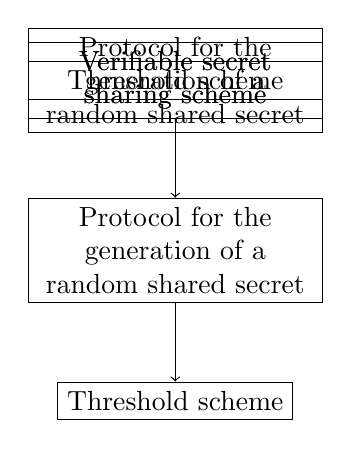
\begin{tikzpicture}[
					every node/.style = {% is not necessary, default node's shape is rectangle
						align=center}
					]	
					
					\node () at (0,0) {};
					\onslide<1-3>{\node[align = center, draw, text width=3.5cm] (a) {Verifiable secret sharing scheme};}
					\onslide<2-3>{\node[align = center, draw, below=of a, text width=3.5cm] (b) {Protocol for the generation of a random shared secret};}
					\onslide<3>{\node[align = center, draw,, below=of b] (c) {Threshold scheme};}
					
					
					\onslide<2-3>{\draw[->] (a) -- (b);}
					\onslide<3>{\draw[->] (b) -- (c);}
					
					\onslide<4-12>{\node[align = center, draw, text width=3.5cm] (a) {Verifiable secret sharing scheme};}
					\onslide<13-17>{\node[align = center, draw, text width=3.5cm] (a) {Protocol for the generation of a random shared secret};}
					\onslide<18-23>{\node[align = center, draw, text width=3.5cm] (a) {Threshold scheme};}
					\end{tikzpicture}}
			\end{textblock*}
			\begin{textblock*}{6cm}(0.3cm,2.5cm) 
				\only<4-9>{
					The dealer:
					\only<5-6>{
						\begin{itemize}
							\item<5-6> {generates secret $r$ and $r' \xleftarrow{\text{\$}} \{1, ..., n - 1\}$;}
							\item<6> {commits to them through the Pedersen commitment $C_0 = rG + r'H$: $C_0$ is broadcast.}
					\end{itemize}}
					\only<7->{
						\begin{itemize}
							\item<7-> {chooses random polynomials:\\
								$f(u) = r + f_1u + ... + f_{t - 1}u^{t - 1}$,\\
								$f'(u) = r' + f_1'u + ... + f_{t - 1}'u^{t - 1}$,\\
								$f_j, \ f_j' \xleftarrow{\text{\$}} \{1, ..., n - 1\}$;}
							\item<8-> computes $(s_i, s_i') = (f(i) \ (\text{mod \ n}), f'(i) \ (\text{mod \ n}))$, \\ $i \in \{1, ..., m\}$ and sends them secretly to $P_i$;
							\item<9-> broadcasts the commitment to the sharing polynomials: $C_j = f_jG + f_j'H$,\\ $j \in \{1, ..., t - 1\}$.
					\end{itemize}}
				}
				\only<10-12>{
					The participants:
					\only<11-12>{
						\begin{itemize}
							\item<11-> verify the consistency of their shares of secret: $s_iG + s_i'H = \sum_{j = 0}^{t - 1}i^jC_j$;
							\item<12-> to reconstruct the secret they rely on Lagrange's interpolation formula: \\
							$f(u) = \sum_{i} f(i)\omega_i(u)$, where $\omega_i(u) = \prod_{j \neq i} \frac{u - j}{i - j} \ (\text{mod} \ n)$.
							\\
							$r = f(0) = \sum_{i}s_i\omega_i$, with $\omega_i = \omega_i(0) = \prod_{j \neq i} \frac{j}{j - i} \ (\text{mod} \ n)$.
						\end{itemize}
					}
				}
			\end{textblock*}
			\begin{textblock*}{6cm}(0.3cm,2.8cm) 
				\only<13-17>{
					Each participant:
					\only<14-17>{
						\begin{itemize}
							\item<14-17> acts as the dealer in the previous protocol ($f_i(u) = \sum_{j = 0}^{t - 1}a_{ij}u^j$, $a_{i0} = r_i$);
							\item<16-17> the shared secret is $r = \sum_{i = 1}^{m}r_i \ (\text{mod} \ n)$ with shares $s_i = \sum_{j = 1}^{m} f_j(i) \ (\text{mod} \ n)$;
							\item<17> broadcast his share of the public key $R_j = r_jG$ ($R = \sum_{j = 1}^{m}R_j = \sum_{j = 1}^{m}r_jG = rG$).
						\end{itemize}
					}
				}
			\end{textblock*}
			\begin{textblock*}{6cm}(0.3cm,2.2cm) 
				\only<18-19>{
					After having established a distributed key pair $(\alpha_1, ..., \alpha_m) \xleftrightarrow{\text{(t, m)}} (q|Q)$ through the protocol for the generation of a random shared secret (that acts as key generation protocol) the signers:
					\only<18-19>{
						\begin{itemize}
							\item<19> run again the same protocol to produce a nonces pair: $(\beta_1, ..., \beta_m) \xleftrightarrow{\text{(t, m)}} (k|K)$.
						\end{itemize}
					}
				}
				\only<20-23>{
					Then each signer $i$:
					\begin{itemize}
						\item<20-23> checks whether $\text{jacobi}(y_K) \neq 1$; if it is the case she sets $\beta_i = n - \beta_i$;
						\item<21-23> reveals her partial signature: $\gamma_i  = \beta_i + e\alpha_i \ (\text{mod} \ n)$, with $e = \text{hash}(x_K||Q||msg)$;
						\item<22-23> computes $\sigma = \sum_{j = 1}^{t} \gamma_j\omega_j \ (\text{mod} \ n)$, with $\omega_j = \prod_{h \neq j} \frac{h}{h - j} \ (\text{mod} \ n)$: $\sigma$ is such that $\sigma = k + eq \ (\text{mod} \ n)$;
						\item<23> the signature is $(x_K, \sigma)$.
					\end{itemize}
					
				}
			\end{textblock*}
			
		\end{column}
		\begin{column}{0.65\linewidth}
			\begin{tikzpicture}[
			every node/.style = {% is not necessary, default node's shape is rectangle
				align=center}
			]	
			
			\node () at (0,0) {};
			\onslide<1-17> {\node(a) [yshift=2cm] {\includegraphics[scale=0.16]{images/Alice.jpg}};}
			\onslide<1-3> {\node (b) [text width=3cm, above=of a, yshift=-1cm, xshift=-0.1cm] {Alice};}
			\onslide<4-12> {\node (b) [text width=3cm, above=of a, yshift=-1cm, xshift=-0.1cm] {Dealer: Alice};}
			\onslide<13-17> {\node (b) [text width=3cm, above=of a, yshift=-1cm, xshift=-0.1cm] {1: Alice};}
			\only<18-23> {\node(a) [yshift=2cm] {\includegraphics[scale=0.16]{images/Alice.jpg}};}
			\only<18-23> {\node (b) [text width=3cm, above=of a, yshift=-1cm, xshift=-0.1cm] {1: Alice};}
			
			\onslide<1-17> {\node (d) [below=of a, xshift = -1.75cm] {\includegraphics[scale=0.21]{images/Bob.jpg}};}
			\onslide<1-3> {\node (e) [text width=3cm, below=of d, yshift=1cm, xshift=0.2cm] {Bob};}
			\onslide<4-12> {\node (e) [text width=3cm, below=of d, yshift=1cm, xshift=0.2cm] {1: Bob};}
			\onslide<13-17> {\node (e) [text width=3cm, below=of d, yshift=1cm, xshift=0.2cm] {2: Bob};}
			
			\onslide<1-17> {\node (g) [below=of a, xshift=1.75cm] {\includegraphics[scale=0.16]{images/Charlotte.jpg}};}
			\onslide<1-3> {\node (h) [text width=3cm, below=of g, yshift=1cm] {Charlotte};}
			\onslide<4-12> {\node (h) [text width=3cm, below=of g, yshift=1cm] {2: Charlotte};}
			\onslide<13-17> {\node (h) [text width=3cm, below=of g, yshift=1cm] {3: Charlotte};}
			\only<18-23> {\node (g) [below=of a] {\includegraphics[scale=0.16]{images/Charlotte.jpg}};}
			\only<18-23> {\node (h) [text width=3cm, below=of g, yshift=1cm] {3: Charlotte};}
			
			\only<5> {\node [right=of a, xshift=-1.45cm, yshift=0.5cm] {$r, r'$};}
			\only<6>{\draw[->] (a) -- (d);
				\draw [->] (a) -- (g);
				\node [right=of a, xshift=-1.5cm, yshift=-1.7cm] {$C_0$};
				\node [right=of a, xshift=-3.8cm, yshift=-1.7cm] {$C_0$};};
			\only<7> {\node [right=of a, xshift=-1.45cm, yshift=0.5cm] {$f, f'$};}
			\only<8>{\draw[->] (a) -- (d);
				\draw [->] (a) -- (g);
				\node [right=of a, xshift=-1.5cm, yshift=-1.7cm] {$(s_2, s_2')$};
				\node [right=of a, xshift=-4.5cm, yshift=-1.7cm] {$(s_1, s_1')$};}
			\only<9>{\draw[->] (a) -- (d);
				\draw [->] (a) -- (g);
				\node [right=of a, xshift=-1.5cm, yshift=-1.7cm] {$C_j$};
				\node [right=of a, xshift=-3.8cm, yshift=-1.7cm] {$C_j$};};
			\only<11> {\node [above=of d, xshift=1.75cm, yshift=-1.6cm] {\includegraphics[scale=0.07]{images/pensiero}};}
			\only<12>{\draw [->] (d) -- (g);
				\draw [->] (g) -- (d);
				\node [right=of d, xshift=-0.8cm, yshift=0.3cm] {$s$};};
			
			\only<14-15>{\node [right=of a, xshift=-1.4cm, yshift=0.3cm] {$r_1, r_1'$};
				\node [right=of a, xshift=-1.4cm, yshift=-0.2cm] {$f_1, f_1'$};
				\node [right=of d, xshift=-1.5cm, yshift=0.3cm] {$r_2, r_2'$};
				\node [right=of d, xshift=-1.5cm, yshift=-0.2cm] {$f_2, f_2'$};
				\node [right=of g, xshift=-1.4cm, yshift=0.3cm] {$r_3, r_3'$};
				\node [right=of g, xshift=-1.4cm, yshift=-0.2cm] {$f_3, f_3'$};};
			\only<15>{\draw [->] (a) -- (d);
				\draw [->] (d) -- (a);
				\draw [->] (a) -- (g);
				\draw [->] (g) -- (a);
				\draw [->] (d) -- (g);
				\draw [->] (g) -- (d);};
			\only<16>{\node [right=of a, xshift=-1.4cm, yshift=0.3cm] {$s_1$};
				\node [right=of d, xshift=-1.5cm, yshift=0.3cm] {$s_2$};
				\node [right=of g, xshift=-1.4cm, yshift=0.3cm] {$s_3$};};		 
			\only<17>{\draw [->] (a) -- (d);
				\draw [->] (d) -- (a);
				\draw [->] (a) -- (g);
				\draw [->] (g) -- (a);
				\draw [->] (d) -- (g);
				\draw [->] (g) -- (d);
				\node [right=of a, xshift=-1.5cm, yshift=-1.7cm] {$R_1$};
				\node [right=of a, xshift=-3.9cm, yshift=-1.7cm] {$R_1$};
				\node [right=of a, xshift=-3.25cm, yshift=-1.8cm] {$R_2$};
				\node [right=of a, xshift=-2.1cm, yshift=-1.8cm] {$R_3$};
				\node [right=of d, xshift = -0.9cm, yshift = 0.3cm] {$R_2$};
				\node [left=of g, xshift = 0.9cm, yshift = -0.3cm] {$R_3$};
			};
			\only<18>{\node [right=of a, xshift=-1.4cm, yshift=0.3cm] {$\alpha_1$};
				\node [right=of g, xshift=-1.4cm, yshift=0.3cm] {$\alpha_3$};
				\draw [->] (a) -- (g);
				\draw [->] (g) -- (a);}
			\only<19>{\node [right=of a, xshift=-1.4cm, yshift=0.3cm] {$\alpha_1, \beta_1$};
				\node [right=of g, xshift=-1.4cm, yshift=0.3cm] {$\alpha_3, \beta_3$};
				\draw [->] (a) -- (g);
				\draw [->] (g) -- (a);}
			\only<21>{
				\draw[transform canvas={xshift=1em}, ->] (a) -- (g);
				\draw[transform canvas={xshift=-1em}, ->] (g) -- (a);
				\node [right=of a, xshift=-2cm, yshift=-2cm] {$\gamma_1$};
				\node [right=of g, xshift=-3.2cm, yshift=2cm] {$\gamma_3$};}
			\only<22>{
				\node [right=of a, xshift=-1.4cm, yshift=0.3cm] {$\sigma$};
				\node [right=of g, xshift=-1.4cm, yshift=0.3cm] {$\sigma$};}
			\only<23>{
				\node [right=of a, xshift=-1.4cm, yshift=0.3cm] {$(x_K, \sigma)$};
				\node [right=of g, xshift=-1.4cm, yshift=0.3cm] {$(x_K, \sigma)$};}
			\end{tikzpicture}
		\end{column}
	\end{columns}
\end{frame}

\begin{frame}[t, label = atomic_swap]
\frametitle{Cross-chain atomic swaps via adaptor signatures}
\begin{tikzpicture}[
every node/.style = {% is not necessary, default node's shape is rectangle
	align=center}
]

\onslide<1->{
	\node () at (0,0) {};
	\node (b1) {\includegraphics[scale=0.1]{images/blockchain.png}};
	
	\node (a) [right=of b1] {\includegraphics[scale=0.15]{images/Alice.jpg}};
	\node (b) [text width=3cm, below=of a, yshift=1cm] {Alice};
	
	\node (d) [right=of a] {\includegraphics[scale=0.2]{images/Bob.jpg}};
	\node (e) [text width=3cm, below=of d, yshift=1cm] {Bob};
	
	\node (b2) [right=of d] {\includegraphics[scale=0.1]{images/blockchain.png}};
	
	\node<1-11> (btc) [above=of b1, yshift = -1cm]{\includegraphics[scale=0.05]{images/bitcoin.png}};
	\node<12-> () [above=of b1, yshift = -1cm]{\includegraphics[scale=0.05]{images/ethereum.png}};
	\node<1-11> (eth) [above=of b2, yshift = -1cm]{\includegraphics[scale=0.05]{images/ethereum.png}};
	\node<12-> () [above=of b2, yshift = -1cm]{\includegraphics[scale=0.05]{images/bitcoin.png}};
	
	\only<2-11>{
		\node () [right=of a, xshift = -4.4cm, yshift=1cm] {$Q_A, Q_A'$};
		\node () [right=of d, xshift = -1.8cm, yshift=1cm] {$Q_B, Q_B'$};}
	\node<3> () [right=of a, xshift = -1.7cm, yshift = 1.2cm] {\includegraphics[scale=0.1]{images/fumetto.png}};
	\only<4-11>{
		\node () [right=of a, xshift = -4.5cm, yshift = 0.4cm] {$Q, Q'$};
		\node () [right=of d, xshift = -1.7cm, yshift = 0.4cm] {$Q, Q'$};}
	\onslide<4-11>{\node (tx1) [draw, below=of b, yshift=0.7cm] {TX$_1$};
		\node<6->[right=of tx1, xshift = -1.15cm, yshift = 0.15cm] (z) {$\xrightarrow{Q}{}$};
		\node<5->[right=of tx1, xshift = -3.15cm, yshift = 0.15cm] (z) {$\xrightarrow{1 \ \text{BTC}}{}$};
		\only<7-9>{\node (refund) [draw, right=of tx1, xshift =-0.55cm] {REF$_1$};
			\node<8-9>[right=of refund, xshift = -1.15cm, yshift = 0.2cm] (z) {$\xrightarrow{Q_A}{}$};
			\node<9> (sig1) [below=of refund, yshift = 1cm, xshift = -0.5cm] {\includegraphics[scale=0.07]{images/sig.jpg}};
			\node<9> (sig2) [below=of refund, yshift = 1cm, xshift = 0.5cm] {\includegraphics[scale=0.05]{images/bob_sig.png}};
			\node<9> () [right=of a, xshift = -1.7cm, yshift = 1.2cm] {\includegraphics[scale=0.1]{images/musig.png}};
		}
		
		\onslide<10->{\node (sig1) [below=of tx1, yshift = 1cm] {\includegraphics[scale=0.1]{images/sig.jpg}};
			\only<11>{\draw[->] (tx1)--(b1);}}
	}
	\only<4-6,10-11>{
		\node (tx2) [draw, below=of e, yshift=0.8cm] {TX$_2$};
		\node<6->[right=of tx2, xshift = -1.15cm, yshift = 0.2cm] (z) {$\xrightarrow{Q'}{}$};
		\node<5->[right=of tx2, xshift = -3.15cm, yshift = 0.15cm] (z) {$\xrightarrow{1 \ \text{ETH}}{}$};
		\onslide<10->{\node (sig1) [below=of tx2, yshift = 1cm, xshift=0.2cm] {\includegraphics[scale=0.06]{images/bob_sig.png}};
			\only<11->{\draw[->] (tx2)--(b2);}}
	}
	\only<12->{
		\node (tx1) [draw, below=of e, yshift=0.8cm, xshift = -1cm] {TX$_1$};
		\node[right=of tx1, xshift = -1.15cm, yshift = 0.2cm] (z) {$\xrightarrow{Q}{}$};
		\node<13-> (tx3) [draw, right=of tx1, xshift = -0.3cm] {TX$_3$};
		\node<14->[right=of tx3, xshift = -1.15cm, yshift = 0.2cm] (z) {$\xrightarrow{Q_B}{}$};
		\node (tx2) [draw, below=of b, yshift=0.7cm, xshift = -1.5cm] {TX$_2$};
		\node[right=of tx2, xshift = -1.15cm, yshift = 0.2cm] (z) {$\xrightarrow{Q'}{}$};
		\node<13-> (tx4) [draw, right=of tx2, xshift = -0.4cm] {TX$_4$};
		\node<14->[right=of tx4, xshift = -1.15cm, yshift = 0.2cm] (z) {$\xrightarrow{Q_A'}{}$};
		\node<15> () [right=of a, xshift = -1.7cm, yshift = 1.2cm] {\includegraphics[scale=0.1]{images/musig_adaptor}};
		\node<16-> (z1) [below=of tx4, yshift = 1cm, xshift = -0.4cm] {\includegraphics[scale=0.07]{images/ethereum_sig.jpg}};
		\node<16-22> (z2) [below=of tx4, yshift = 1cm, xshift = 0.21cm] {\includegraphics[scale=0.05]{images/half_bob}};
		\node<16-> (z3) [below=of tx3, yshift = 1cm, xshift = -0.4cm] {\includegraphics[scale=0.07]{images/bitcoin_sig.jpg}};
		\node<16-18> (z4) [below=of tx3, yshift = 1cm, xshift = 0.21cm] {\includegraphics[scale=0.05]{images/half_bob}};
		\node<16-17> () [right=of e, xshift = -1.7cm, yshift = 2 cm] {t};
		\node<18> () [right=of z4, xshift = -1.2cm] {+ t};
		\node<19-> (sig2) [below=of tx3, yshift = 1cm, xshift = 0.5cm] {\includegraphics[scale=0.05]{images/bob_bitcoin.png}};
		\draw<20-> [->] (tx3)--(b2);
		\node<21>() [right=of a, xshift = -2cm, yshift=1.3cm] {\includegraphics[scale=0.065]{images/adaptor}};
		\node<22> () [right=of z2, xshift = -1.2cm] {+ t};
		\node<23-> (sig2) [below=of tx4, yshift = 1cm, xshift = 0.5cm] {\includegraphics[scale=0.05]{images/bob_ethereum.png}};
		\draw<24-> [->] (tx4)--(b1);
	}
}
\end{tikzpicture}
\only<1>{\centering \textcolor{white}{WAAA}\par}
\only<2> {\centering The participants have a key pair for each chain:\\ $\{q_A, Q_A\}$, $\{q_A', Q_A'\}$, $\{q_B, Q_B\}$, $\{q_B', Q_B'\}$.\par}
\only<3> {\centering According to the MuSig protocol they construct the aggregated public keys:\\ $Q = \text{hash}(\langle Q_A, Q_B \rangle || Q_A)Q_A +  \text{hash}(\langle Q_A, Q_B \rangle || Q_B)Q_B,$\\ 
	$Q' = \text{hash}(\langle Q_A', Q_B' \rangle || Q_A')Q_A' +  \text{hash}(\langle Q_A', Q_B' \rangle || Q_B')Q_B'$.\par}
\only<4-6> {\centering They start constructing transactions on the respective chain: 
	\begin{itemize}
		\item<5-> They agree on the exchange rate;
		\item<6-> The funds are locked with the aggregated public keys. 
	\end{itemize}
	\par}
\only<7-9> {\centering Before signing, they construct a refund transaction (here Alice's example). Both transactions have to be time locked and the time lock over Bob's transaction has to be greater.
	\only<9> {To sign it, the participants have to interact via the MuSig protocol.}\par}
\only<10-11> {\centering Having the refund transactions, Alice and Bob can confidently sign TX$_1$ and TX$_2$.
	\only<11>{Then they broadcast them and wait for confirmation.}\par}
\only<12-15>{\centering At this point they construct transactions to grab the other coin:
	\only<15>{they need to resort to the MuSig protocol to generate valid signatures; to ensure atomicity, Bob produces two adaptor signatures using the same secret value $t$.}\par}
\only<16>{\centering Alice has to check that the two signatures are valid adaptor signatures and that it has been used the same secret value.\par}
\only<17>{\centering This results in two partial (invalid) signatures: $(x_{K_A + K_B + T}, \tilde{s})$ and $(x_{K_A' + K_B' + T}, \tilde{s}')$, with $\tilde{s} = k_A + k_B + \text{hash}(x_{K_A + K_B + T}||Q||\text{TX}_3)(q_A + q_B)$ and $\tilde{s}' = k_A' + k_B' + \text{hash}(x_{K_A' + K_B' + T}||Q'||\text{TX}_4)(q_A' + q_B' )$.\par}
\only<18-19>{\centering Whenever Bob wants to take the coins he can add $t$ to the adaptor signature, making it valid: $(x_{K_A  + K_B + T}, \tilde{s} + t)$.\par}
\only<20>{\centering Now he can broadcast to the blockchain.\par}
\only<21>{\centering Monitoring the blockchain Alice sees the valid signature: subtracting from it the adaptor signature she learns the secret $t$. \par}
\only<22-23>{\centering  Adding it to the other adaptor signature results again in a valid signature for TX$_4$. \par}
\only<24>{\centering She can now broadcast it to the blockchain: this concludes the protocol. \par}
\end{frame}

	\backupend
\end{document}
